\documentclass[11pt]{amsart}
\usepackage{amsmath,amssymb,amsthm}
\usepackage[margin=1.1in]{geometry}
\usepackage{microtype}
\usepackage{enumitem}
\usepackage{array}
\usepackage{booktabs}
\usepackage{graphicx}
\usepackage{float}
\graphicspath{{../figures/}}
\usepackage[colorlinks=true,linkcolor=blue,citecolor=blue,urlcolor=blue]{hyperref}
\emergencystretch=2.5em
\raggedbottom

\newtheorem{theorem}{Theorem}[section]
\newtheorem{lemma}[theorem]{Lemma}
\newtheorem{proposition}[theorem]{Proposition}
\newtheorem{corollary}[theorem]{Corollary}
\newtheorem{conjecture}[theorem]{Conjecture}
\theoremstyle{remark}
\newtheorem{remark}[theorem]{Remark}

\newcommand{\Z}{\mathbb{Z}}
\newcommand{\HH}{\mathbb{H}}
\newcommand{\cA}{\mathcal{A}}
\newcommand{\cB}{\mathcal{B}}
\newcommand{\e}{\varepsilon}
\newcommand{\dd}{\mathrm{d}}
\DeclareMathOperator{\pr}{pr}
\DeclareMathOperator{\vol}{vol}
\DeclareMathOperator{\tr}{tr}

\title[Sums of two squares with few prime factors, III]{Sums of two squares with few prime factors, III:\\ the dispersion obstacle, sieve barriers at the level $1/2$,\\ and short-interval mean squares}
\author{Ruqing Chen}
\address{GUT Geoservice Inc., Montreal, Canada}
\email{ruqing@hotmail.com}
\date{\today\ (draft)}

\begin{document}

\begin{abstract}
Parts I and II of this series proved the level of distribution $1/2$ for the weighted sequence $r(n)r(N-n)$ through the theta series $\theta^2(mz)\theta^2(m'z)$ of quaternary forms, and with it $\Omega(n(N-n))\le7$, $\max(\Omega(n),\Omega(N-n))\le5$ for every large $N\equiv2\pmod 4$, with $n$ and $N-n$ sums of two squares. This part examines the three questions these results leave open, and answers them to the extent that the present methods allow. (1)~The remainder $R_d=\sum_{d_1d_2=d}R(d_1,d_2;N)$ that the two-dimensional sieve uses is the coefficient of the projection of the cusp form $G_{t,d}$ onto the joint $(+1)$-eigenspace of the Atkin--Lehner involutions $W_p$, $p\mid d$ (an exact identity $\sum_{u\mid d}G_{tu,d/u}=\prod_{p\mid d}(1+W_p)G_{t,d}$), so that every Hecke component with $\eta_p(f)=-1$ for some $p\mid(d,M_1)$ cancels, in particular every oldform of odd level in the terms of smallest level; numerically the cancellation is of square-root strength and no more, a $d^{o(1)}$ gain. (2)~The remainder sum $\sum\lambda_d\lambda'_eR(d,e;N)$ has as its leading term a trilinear form in classical Kloosterman sums $S(\overline{16m}N,|h|^2;m'k)$ over the moduli $c\equiv0\pmod{m'}$ (the Fourier transform of the circle $x^2+y^2\equiv a$ modulo any odd $c$ is a classical Kloosterman sum, and the character $\chi_{-4}$ cancels exactly); the uniform bound of Part~I is equivalent to square-root cancellation in the sum over $k$, square-root cancellation over $m'$ would give the level $2/3$, and the single fixed argument $N$, carried by the unit $\overline{16m}$ modulo the modulus, is, in every assignment of Drappeau's bound and in every Cauchy--Schwarz and Poisson arrangement, the term that blocks a level beyond $1/2$. (3)~The weights $r(n)r(N-n)$ cost the sieve dimension, $2$ against $1$; Selberg-type mollifiers truncated below the sifting limit are identically $1$ on the sifted integers, mollifiers reaching the Richert range cost more level than they return, and a linear programme over all non-negative weight functions, separable or with a term for each pair of prime factors, finds Richert's linear weight optimal on the grid, so that the gap of $0.030$ to $(7,4)$ is structural. (4)~In every interval $(X,X+X^\Delta]$ with $\Delta>1/2$, almost all $N$ have the level of distribution $\Delta-\e$ (unconditionally); a short-interval mean square $\sum_{X<n\le X+H}|a_G(n)|^2\ll X^\eta(H+L)X\|G\|^2/L$ would raise it to $(1+\Delta)/2$ for every $\Delta>0$, and the same bound without the term $L$, for the theta forms alone, to $1-\e$; the latter interpolates between the individual conjecture of Part~II at $H=1$ and its mean-square theorem at $H=X$, and the data support it down to $H=16$. Spectrally, the diagonal of the Hecke expansion satisfies the conjectured bound unconditionally for every $H\ge X^\e$ (Deligne, Shiu, Hoffstein--Lockhart, and the Rankin--Selberg formula of Part~II for the oldform components), so that the conjecture is exactly the cancellation of the off-diagonal; the term $L$ is the coherence of the Poincar\'e series, whose spectral coefficients align at a single $n$, while the spectral coefficients of the theta forms are central values independent of the window, and their off-diagonal correlations average out, which is what the data show. The lattice-point form of the variance does not avoid this: the precision it requires lies below the floor of every circle-method error term. The Kloosterman form of the remainder factors, by the Chinese remainder theorem, into a bilinear form in the two moduli $(k,m')$ in which the fixed argument enters as $\overline{16m}N\bar k$ modulo $m'$; this is the shape in which a saving over the sieve modulus would have to be found.
\end{abstract}

\maketitle

\section{Introduction and statement of results}\label{sec:intro}

\subsection{Setting}
We keep the notation of Parts I and II \cite{ChenI,ChenII}: $\chi=\chi_{-4}$, $r(n)=4\sum_{k\mid n}\chi(k)$, $\Theta_{m,m'}=\theta^2(mz)\theta^2(m'z)=E_{m,m'}+G_{m,m'}\in M_2(\Gamma_0(4mm'))$ for coprime odd $m,m'$ with Eisenstein part $E$ and cuspidal part $G$, $a_{G}(N)=T(m,m';N)-M(m,m';N)$ with $T(m,m';N)=\sum_{m\alpha+m'\beta=N}r(\alpha)r(\beta)$ and $M$ the Siegel main term, $W_Q$ the Atkin--Lehner matrices, $\eta_Q(f)$ the eigenvalues of the newforms, and $(f|_k\gamma)(z)=(\det\gamma)^{k/2}(cz+d)^{-k}f(\gamma z)$, so that scalar matrices act trivially. For $N\equiv2\pmod4$, $\cA=\{n\le N:(n,N)=1\}$, $w(n)=r(n)r(N-n)$, and for coprime square-free $d_1,d_2$ with $(d_1d_2,2N)=1$,
\[
S(d_1,d_2)=\sum_{\substack{n\in\cA\\ d_1\mid n,\ d_2\mid N-n}}w(n)=X_Nh(d_1)h(d_2)+R(d_1,d_2;N),\qquad R_d=\sum_{d_1d_2=d}R(d_1,d_2;N),
\]
with $h(p)=(2p-1)/(p(p+1))$ for $p\equiv1$, $h(q)=1/(q(q-1))$ for $q\equiv3\pmod4$ (Part~I, Section~3; Part~II, Section~7.2). By Part~I, (16) (Part~II, (4)),
\begin{multline}\label{eq:Rdecomp}
R(d_1,d_2;N)=\sum_{t\mid N^\flat}\mu(t)\sum_{\substack{t_1=tu\\ u\mid t}}c_t(t_1)\sum_{\substack{s_1\mid d_1\\ s_2\mid d_2}}c_{d_1}(d_1s_1)c_{d_2}(d_2s_2)\bigl(a_G(N)-a_G(N/2)\bigr),\\ G=G_{t_1d_1s_1,\,d_2s_2},
\end{multline}
where $c_p(p)=2$, $c_p(p^2)=-1$ for split $p$ and $c_q(q)=0$, $c_q(q^2)=1$ for inert $q$, multiplicatively; every parameter $t_1d_1s_1$, $d_2s_2$ is $\equiv1\pmod4$, being a product of split primes and of squares of inert primes. Part~I proved $\|G_{m,m'}\|^2\ll(mm')^\e$ and $|a_G(N)|\ll d(N)N^{1/2}(mm')^\e$, hence the level of distribution $1/2$ for $w$ (Part~I, Theorem~3.2); Part~II proved the mean-square bound $\sum_{n\le Y}|a_G(n)|^2\le4\pi e^2Y(1+54Y/L)\|G\|^2$ for every $G\in S_2(\Gamma_0(L))$ (Theorem~1.2 there), the level $1-\e$ for almost all $N$ (Theorem~1.3), the asymptotic formula $\|G_{m,m'}\|^2\sim\frac1\pi\sum_{\delta\mid mm',\,\delta^2<mm'}\delta^{-1}(\log(mm'/\delta^2))^2$, the explicit Rankin--Selberg formula $\langle\Theta_{1,n},f(d\,\cdot)\rangle=\pm\frac4{\pi^2}2^{\omega(n/M_1)}d^{-1}L(1,f)L(1,f\otimes\chi)$ (Theorem~6.7), and, with the two-dimensional sieve of Diamond, Halberstam and Richert, the pair $(7,5)$ for every large $N\equiv2\pmod4$ (Theorem~7.1).

\subsection{The three questions}
Those results leave three questions.
\begin{enumerate}[label=\textup{(\roman*)},leftmargin=2.2em]
\item Can the level of distribution for \emph{every} $N$ be pushed beyond $1/2$ by cancellation in the sum over the moduli, as the dispersion method does for primes in progressions?
\item At the level $1/2$, can the pair $(7,5)$ of Part~II be improved to $(7,4)$, which the two-dimensional sieve misses by $0.030$ in the margin, by using the symmetry of the remainder, by mollifying the weights, or by changing the shape of Richert's weight?
\item What is the level of distribution for almost all $N$ in a short interval $(X,X+X^\Delta]$, between the single-$N$ level $1/2$ and the almost-all level $1-\e$ of Part~II?
\end{enumerate}
This paper answers (i) and (ii) negatively within the present methods, with an exact description of the obstruction in each case, and answers (iii) unconditionally for $\Delta>1/2$ and conditionally, on a precisely identified short-interval mean square, for every $\Delta>0$.

\subsection{Results}
\emph{The symmetric remainder} (Section~\ref{sec:symmetric}). Lemma~\ref{lem:transport} moves any part of the parameter $m$ of $\Theta_{m,m'}$ to the other side by an Atkin--Lehner involution, and Proposition~\ref{prop:sym} gives, for odd square-free $d$,
\[
\sum_{u\mid d}G_{t_1u_s,(d/u)_s}=2^{\omega(d)}P^+_{d,s}G_{t_1,ds},
\]
with $P^+_{d,s}$ the projection onto the joint $(+1)$-eigenspace of the $W_{p^{v_p(ds)}}$, $p\mid d$. So the remainder $R_d$ of the two-dimensional sieve is, term by term, the coefficient of this projection (Corollary~\ref{cor:Rd}), and in the terms of smallest level every Hecke component on which some $W_p$, $p\mid d$, acts by $-1$ cancels exactly, in particular every oldform of odd level (Proposition~\ref{prop:cancel}). Numerically the cancellation is of square-root strength and no more, because the norm of $G_{1,d}$ is close to equidistributed over the joint eigenspaces (Section~\ref{subsec:symnum}, Figure~\ref{fig:sym}); it is a $d^{o(1)}$ gain and does not move the level.

\emph{The dispersion form} (Sections~\ref{sec:dispersion}--\ref{sec:poisson}). The Fourier transform of the circle $x^2+y^2\equiv a$ modulo any odd $c$ is a classical Kloosterman sum (Lemma~\ref{lem:circle}), and the remainder $a_G(N)-a_G(N/2)$ has as its leading term a sum of $S(\overline{16m}N,|h|^2;m'k)$ over the moduli $m'k$, in which the character $\chi_{-4}$ of the divisor expansion is cancelled exactly by the sign of the Gauss sums (Proposition~\ref{prop:dispersion}). The uniform bound of Part~I is equivalent to square-root cancellation in the sum over $k$; square-root cancellation over the sieve modulus $m'$ would give the level $2/3$, over $m$ as well the level $1$; the Weil bound gives $1/4$. Substituting the bounds of Deshouillers--Iwaniec and Drappeau in every possible assignment of roles (Section~\ref{subsec:subst}), and applying Cauchy--Schwarz over the smooth variables with Poisson summation in the dual variable $h$ (Section~\ref{sec:poisson}), one finds the same obstruction each time: the single fixed argument $N$, carried by the unit $\overline{16m}$ modulo the modulus, which the dual sum cannot remove because the box of $h$ has side $\le\sqrt{mm'}$ while every modulus is $\ge\sqrt N$. The Chinese remainder theorem factors the Kloosterman sums and writes the remainder as a bilinear form in the two moduli $(k,m')$, in which the fixed argument enters modulo $m'$ as $\overline{16m}N\bar k$ (Section~\ref{subsec:bilinear}): this is the shape in which a saving over the sieve modulus would have to be found, bilinear as in the work of Bombieri--Friedlander--Iwaniec and Duke--Friedlander--Iwaniec, and the sum over $k$ alone, whose phases $\bar k\pmod{m'}$ do mix, cannot give more than the theta bound.

\emph{Sieve barriers at the level $1/2$} (Sections~\ref{sec:dimension}--\ref{sec:optimal}). The factor $2^{\Omega(n(N-n))}$ of the weights enters only the constant; what the weights cost is the sieve dimension, $2$ against $1$ for the indicator weights (Section~\ref{subsec:dim}: a dimension-one sieve would give $(5,3)$ at the level $1/2$ and Chen's shape $(3,2)$ from $4/5$ on). A Selberg-type mollifier truncated below the sifting limit is identically $1$ on the sifted integers (Theorem~\ref{thm:nothing}); it changes the density exactly at the primes it contains (Proposition~\ref{prop:density}), so that acting on the Richert range costs more level than it returns, and every partial version is worse than $(7,5)$. A linear programme over all non-negative weight functions $g$, with the exact prime-configuration constraints evaluated by dynamic programming, finds Richert's linear weight optimal on the grid for $(7,5)$, $(7,4)$ and $(6,4)$ (Section~\ref{sec:optimal}, Figure~\ref{fig:barriers}): the gap to $(7,4)$ is not in the shape of the weight. Nor is it in its separability: the sieve accepts weights with a term for each pair of prime factors, sieved at the level $N^{\theta-t_p-t_q}$ (Proposition~\ref{prop:pairsieve}), the programme extends to them, and its solution is again the linear weight with the pair term identically zero, even when every sieve cost $F_2$ is set to $1$; the dual of the programme says why (Proposition~\ref{prop:dual}, Section~\ref{subsec:pairs}). The remaining exit inside the sieve, Chen's switching, leads to the remainder problem of question~(i) with a prime variable inside the modulus (Section~\ref{sec:optimal}, end).

\emph{Short intervals} (Sections~\ref{sec:short}--\ref{sec:spectral}). Theorem~\ref{thm:short}: for $H=X^\Delta$ with $\Delta>1/2$, all but $O(HX^{-\e/4})$ of the $N\equiv2\pmod4$ in $(X,X+H]$ have the level of distribution $\Delta-3\e$, hence $(6,4)$ in every interval of length $X^{2/3+\e}$ and $(5,4)$ in every interval of length $X^{19/20+\e}$. Proposition~\ref{prop:shortcond}: the short-interval mean square $\sum_{X<n\le X+H}|a_G(n)|^2\ll X^\eta(H+L)X\|G\|^2/L$ for all $G\in S_2(\Gamma_0(L))$ would raise the level to $(1+\Delta)/2$ for every $\Delta>0$; it is a large-sieve inequality for the Poincar\'e series of the interval, sharp, and its Kloosterman form is the obstruction of Section~\ref{sec:dispersion} in its symmetric shape. Conjecture~\ref{conj:short} is the same bound without the term $L$ for the theta forms alone; it interpolates between the individual conjecture of Part~II ($H=1$) and the mean-square theorem ($H=X$), it gives the level $1-\e$ for almost all $N$ in every interval of length $X^\Delta$, $\Delta>0$ (Corollary~\ref{cor:short}), and the data support it down to $H=16$ (Figure~\ref{fig:short}). Section~\ref{sec:spectral} explains the difference spectrally: in an orthogonal Hecke basis the mean square splits into a diagonal and an off-diagonal. The diagonal satisfies the bound of Conjecture~\ref{conj:short} unconditionally: eigenform by eigenform up to the scaling $L/M$ of the oldforms of level $M$ (Theorem~\ref{prop:diag}: Deligne's bound, Shiu's theorem on $\sum_{X<n\le X+H}d(n)^2$, and the lower bound $\|\varphi\|^2\gg L^{1-\e}$ for the Petersson norms), and in full for the theta forms and every $H\ge X^\e$, because their oldform components of small level have small norm by the Rankin--Selberg formula of Part~II (Proposition~\ref{prop:diagtheta}); so that Conjecture~\ref{conj:short} is equivalent to the cancellation of the off-diagonal (Corollary~\ref{cor:equiv}), and the trivial spectral bound, which at $H=1$ is the uniform bound of Part~I, exceeds it by exactly the factor $L$ (Remark~\ref{rem:trivial}). The off-diagonal is coherent for the Poincar\'e series and is a sum of short-interval correlations of distinct eigenforms, with window-independent coefficients, for the theta forms (Proposition~\ref{prop:mechanism}); numerically the off-diagonal of $G_{1,q}$ averages to zero and stays below the diagonal (Table~\ref{tab:spectral}). Finally, the lattice-point form of the variance, $\sum_{N\in I}(T-M)^2$ as a count of zeros of $Q\oplus(-Q)$ in eight variables, does not avoid the spectral problem: it needs a twisted first moment of $a_G$ with square-root cancellation, and the precision $HX/L$ it requires lies below the floor $X^2\|G\|^2/L$ of every circle-method error term (Proposition~\ref{prop:lattice}, Section~\ref{subsec:lattice}).

What is proved and what is not. Lemma~\ref{lem:transport}, Propositions~\ref{prop:sym}, \ref{prop:cancel}, Lemma~\ref{lem:circle}, Proposition~\ref{prop:dispersion}, Theorems~\ref{thm:nothing}, \ref{thm:short} and \ref{prop:diag}, Propositions~\ref{prop:density}, \ref{prop:pairsieve}, \ref{prop:dual}, \ref{prop:shortcond}, \ref{prop:diagtheta}, \ref{prop:mechanism}, \ref{prop:lattice}, and Corollaries~\ref{cor:short} and \ref{cor:equiv} are theorems (Proposition~\ref{prop:shortcond} and Corollary~\ref{cor:short} conditional on the stated hypotheses). The exponent bookkeeping of Sections~\ref{subsec:book}--\ref{subsec:subst} and \ref{sec:poisson} is carried out for the leading term of Proposition~\ref{prop:dispersion} under the most favourable assumptions, and establishes what a proof would have to beat, not a theorem; the optimality of Richert's weight among the separable and the pair weights (Section~\ref{sec:optimal}) is the solution of linear programmes on a grid; and the comparisons with random signs, the eigenspace shares and the short-interval ratios are numerical observations on the stated data.

\section{The symmetric remainder and the Atkin--Lehner projection}\label{sec:symmetric}

\subsection{Transport of a factor by an Atkin--Lehner involution}
Lemma~6.1 of Part~II moves the whole factor $m$ of $\Theta_{m,m'}$ to the other side. The same computation moves any part of it.

\begin{lemma}\label{lem:transport}
Let $m_1,m_2,m'$ be pairwise coprime odd positive integers, $L=4m_1m_2m'$ and $W_{m_1}$ an Atkin--Lehner matrix of level $L$. Then
\[
\Theta_{m_1m_2,\,m'}|_2W_{m_1}=\chi(m_1)\,\Theta_{m_2,\,m_1m'},\qquad\text{hence}\qquad G_{m_1m_2,\,m'}=\chi(m_1)\,G_{m_2,\,m_1m'}|_2W_{m_1}.
\]
\end{lemma}
\begin{proof}
Write $W_{m_1}=\left(\begin{smallmatrix}m_1a&b\\Lc&m_1d\end{smallmatrix}\right)$ with $m_1ad-4m_2m'bc=1$; then $d$ is odd. First, $B_{m_1m_2}W_{m_1}=m_1B_{m_2}\gamma$ with $\gamma=\left(\begin{smallmatrix}m_1a&b\\4m_2m'c&d\end{smallmatrix}\right)\in\Gamma_0(4m_2m')\subseteq\Gamma_0(4m_2)$, as one checks by multiplying out; since $\theta^2(m_2\,\cdot)\in M_1(\Gamma_0(4m_2),\chi)$,
\begin{align*}
\theta^2(m_1m_2\,\cdot)|_1W_{m_1}&=(m_1m_2)^{-1/2}\,\theta^2|_1(B_{m_1m_2}W_{m_1})\\
&=(m_1m_2)^{-1/2}\bigl(\theta^2|_1B_{m_2}\bigr)|_1\gamma=m_1^{-1/2}\chi(d)\,\theta^2(m_2z).
\end{align*}
Second, $W_{m_1}=\gamma'B_{m_1}$ with $\gamma'=\left(\begin{smallmatrix}a&b\\4m_2m'c&m_1d\end{smallmatrix}\right)\in\Gamma_0(4m_2m')\subseteq\Gamma_0(4m')$, so
\[
\theta^2(m'\cdot)|_1W_{m_1}=\chi(m_1d)\,\theta^2(m'\cdot)|_1B_{m_1}=\chi(m_1d)\,m_1^{1/2}\theta^2(m_1m'z).
\]
Multiplying, $\Theta_{m_1m_2,m'}|_2W_{m_1}=\chi(m_1)\theta^2(m_2z)\theta^2(m_1m'z)$. The statement for $G$ follows because $|_2W_{m_1}$ preserves the orthogonal decomposition into Eisenstein and cuspidal parts (Part~II, Section~6.1) and $W_{m_1}^2$ acts trivially.
\end{proof}

\subsection{The sum over the factorisations}
For odd square-free $d$, $s\mid d$ and $u\mid d$ put $u_s=u\,(u,s)$, so that $u_s\,(d/u)_s=ds$ and $u_s$ is the part of $ds$ supported on the primes of $u$.

\begin{proposition}\label{prop:sym}
Let $d$ be odd and square-free, $s\mid d$, and $t_1$ odd with $(t_1,d)=1$. Then
\[
\sum_{u\mid d}G_{t_1u_s,\,(d/u)_s}=G_{t_1,\,ds}\Big|_2\prod_{p\mid d}\bigl(1+\chi(p^{v_p(ds)})\,W_{p^{v_p(ds)}}\bigr),
\]
the $W$'s being Atkin--Lehner matrices of level $4t_1ds$. If every prime power $p^{v_p(ds)}$ is $\equiv1\pmod4$ (which is the case for every term of \eqref{eq:Rdecomp}), the right-hand side is $2^{\omega(d)}P^+_{d,s}G_{t_1,ds}$, where $P^+_{d,s}=\prod_{p\mid d}\frac12(1+W_{p^{v_p(ds)}})$ is the orthogonal projection onto the joint $(+1)$-eigenspace of the commuting involutions $W_{p^{v_p(ds)}}$, $p\mid d$.
\end{proposition}
\begin{proof}
By Lemma~\ref{lem:transport} with $(m_1,m_2,m')=(u_s,t_1,(d/u)_s)$, $G_{t_1u_s,(d/u)_s}=\chi(u_s)G_{t_1,ds}|_2W_{u_s}$. For coprime exact divisors $Q,Q'$ of the level, $W_QW_{Q'}$ is an Atkin--Lehner matrix $W_{QQ'}$ up to a scalar and an element of $\Gamma_0(L)$ \cite{AL}, so $W_{u_s}=\prod_{p\mid u}W_{p^{v_p(ds)}}$ on $M_2(\Gamma_0(L))$, and $\chi(u_s)=\prod_{p\mid u}\chi(p^{v_p(ds)})$. Expanding the product over $p\mid d$ gives the sum over $u\mid d$. The $W_{p^{v}}$ are commuting self-adjoint involutions, so $\frac12(1+W)$ is the orthogonal projection onto the $(+1)$-eigenspace and the product of the projections is the projection onto the intersection.
\end{proof}

\begin{corollary}\label{cor:Rd}
With the notation of \eqref{eq:Rdecomp}, for odd square-free $d$ with $(d,2N)=1$,
\[
R_d=\sum_{t\mid N^\flat}\mu(t)\sum_{t_1=tu,\ u\mid t}c_t(t_1)\sum_{s\mid d}c_d(ds)\,2^{\omega(d)}\Bigl(a_{P^+_{d,s}G_{t_1,ds}}(N)-a_{P^+_{d,s}G_{t_1,ds}}(N/2)\Bigr).
\]
\end{corollary}
\begin{proof}
In \eqref{eq:Rdecomp}, $c_{d_1}(d_1s_1)c_{d_2}(d_2s_2)=c_d(ds)$ with $s=s_1s_2$ by multiplicativity, and for fixed $s$ the pair $(s_1,s_2)$ is determined by $(d_1,d_2)$: $s_1=(s,d_1)$, $s_2=(s,d_2)$. Hence summing \eqref{eq:Rdecomp} over $d_1d_2=d$ sums, for each $(t,t_1,s)$, the coefficients of $G_{t_1(d_1)_s,(d_2)_s}$ over all $d_1\mid d$, and Proposition~\ref{prop:sym} applies.
\end{proof}

\subsection{Which components cancel}
Let now $s=1$, $t_1=1$ (the terms of smallest level, which carry most of the remainder) and $n=d$. For a newform $f$ of level $2^eM_1\mid4d$ let $S(f)=\mathrm{span}\{f(\delta\,\cdot):\delta\mid4d/(2^eM_1)\}$ and $\pr_f$ the orthogonal projection, as in Part~II, Proposition~6.19.

\begin{proposition}\label{prop:cancel}
Let $d$ be odd and square-free.
\begin{enumerate}[label=\textup{(\roman*)},leftmargin=2.2em]
\item If $p\mid M_1$, $W_p$ acts on $S(f)$ as the scalar $\eta_p(f)$. If $p\mid d$, $p\nmid M_1$, $W_p$ maps $f(\delta\,\cdot)$ to $(\delta'/\delta)f(\delta'\cdot)$ with $\delta'=\delta p$ or $\delta/p$ (Part~II, Lemma~6.8), so that $S(f)$ splits into two $W_p$-eigenspaces of equal dimension.
\item $W_d=\prod_{p\mid d}W_p$ acts on $G_{1,d}$ as $\chi(d)$ (Part~II, Remark~6.9(i)).
\item Consequently $P^+_{d,1}\pr_fG_{1,d}=0$ whenever $\eta_p(f)=-1$ for some $p\mid M_1$. In particular, writing $\e(f)=-\eta_{2^e}(f)\eta_{M_1}(f)$ for the root number and using $\eta_4=-1$ for $e=2$ (Part~II, Proposition~6.17) and Theorem~6.7(ii) of Part~II (the component $\pr_fG_{1,d}$ is non-zero only if $L(1,f)L(1,f\otimes\chi)\ne0$, hence only if $\e(f)=+1$):
\begin{itemize}[leftmargin=1.6em]
\item $e=0$, $M_1>1$: $\e(f)=+1$ forces $\eta_{M_1}(f)=-1$, so some $\eta_p(f)=-1$ and the whole component cancels; \emph{every oldform of odd level cancels in $R_d$};
\item $e=1$: $\e(f)=+1$ forces $\eta_{M_1}(f)=-\eta_2(f)$; the component survives only if $\eta_2(f)=-1$, i.e.\ $a_f(2)=+1$, and $\eta_p(f)=+1$ for every $p\mid M_1$;
\item $e=2$: $\e(f)=\eta_{M_1}(f)$, so $\eta_{M_1}(f)=+1$ is automatic, and the component survives iff $\eta_p(f)=+1$ for every $p\mid M_1$; for the newforms of level $4d$ this is the condition $\eta_p=+1$ for all $p\mid d$.
\end{itemize}
What survives of a surviving component is its part in $\bigcap_{p\mid d,\,p\nmid M_1}S(f)^{+,p}$, and it enters $R_d$ with the factor $2^{\omega(d)}$.
\end{enumerate}
\end{proposition}
\begin{proof}
(i) is Lemma~6.8 of Part~II with $Q=p$; (ii) is Lemma~\ref{lem:transport} with $(m_1,m_2,m')=(d,1,1)$ and $\Theta_{d,1}=\Theta_{1,d}$. For (iii), $P^+_{d,1}$ contains the factor $\frac12(1+W_p)$, which annihilates $S(f)$ when $W_p=-1$ on $S(f)$. The sign conditions are the functional equation $\Lambda(s,f)=\e(f)\Lambda(2-s,f)$ with $\e(f)=-\eta_{\mathrm{level}}(f)$ in weight $2$.
\end{proof}

\begin{remark}\label{rem:symrem}
(i) For $d=p$ prime nothing cancels: $W_p=\chi(p)$ on $G_{1,p}$, and indeed $R(p,1)=R(1,p)$ by the symmetry $n\leftrightarrow N-n$ of $w$. The claim that ``all $f$ with $\eta_p(f)=-1$ for some $p\mid(d,M_1)$ cancel'' is correct, but for $d=p$ the set of such $f$ in $G_{1,p}$ is empty. The cancellation is between the $2^{\omega(d)-1}$ \emph{unordered} splittings $\{d_1,d_2\}$; for $d=p_1p_2$ it is between $R(d,1)$ and $R(p_1,p_2)$, i.e.\ between $G_{1,d}$ and $G_{p_1,p_2}=G_{1,d}|W_{p_1}$, and it removes the $(-,-)$-eigenspace, which by (iii) contains all the oldforms of odd level, the oldforms of level $2p_i$ with $a_f(2)=-1$, and half (in the sense of (i)) of every other component, the newforms of level $4d$ with $\eta_{p_1}=\eta_{p_2}=-1$ included.

(ii) The identity of Proposition~\ref{prop:sym} holds for the terms with $s>1$ (parameters with squares of primes) as well; there $W_{p^2}$ acts on $S(f)$ with both eigenvalues even when $p\mid M_1$, and the description (iii) does not apply verbatim. These terms are smaller by $(ds/d)^{-1/2}$ in mean square.

(iii) The corresponding statement for the sum with the weight $\chi(m)$ over all factorisations $m\mid n$ is Proposition~6.19 of Part~II; here $\chi(m)=1$ for every $m$ that occurs, and the point is that the sieve itself performs this sum.
\end{remark}

\subsection{Numerical results}\label{subsec:symnum}
The script \texttt{symmetric\_remainder.py} computes every $R(d_1,d_2;N)$ exactly (direct summation of $w(n)$ over the progression, main term $X_Nh(d_1)h(d_2)$ from Part~I, (17)--(18)) for all admissible pairs with $d_1d_2\le N^{3/4}$ and $24$ values of $N\equiv2\pmod4$ near $2\cdot10^6$ and $3\cdot10^6$, and compares $A_{\mathrm{sym}}=\sum_{d\le D}|R_d|$ with $A_{\mathrm{abs}}=\sum_{d_1d_2\le D}|R(d_1,d_2)|$ and with the random-sign baseline $A_{\mathrm{rnd}}$ (independent signs on the unordered splittings, averaged over $40$ draws). The symmetry $R(d_1,d_2)=R(d_2,d_1)$ holds to $10^{-10}$. (The values of $N$ are $2000002$, $2000006$, $2000018$, $3000002$ and $2000030+4j$, $0\le j<20$; there are about $21000$ moduli $d\le N^{3/4}$ and $107000$ pairs per $N$, of which $569$ moduli have $d\le N^{1/2}$; the random signs use NumPy's generator with the seed $7$; the per-$N$ tables are in the output file. The exact cancellation is the theorem; the comparison with random signs is an observation on these $24$ values of $N$.) Table~\ref{tab:ratios} and Figure~\ref{fig:sym}(a) give the averages over the $24$ values of $N$ (\texttt{results/symmetric\_remainder.txt}).

\begin{table}[htbp]
\centering\small
\begin{tabular}{c|ccc|ccc|c}
\toprule
$\theta$ & \multicolumn{3}{c|}{$A_{\mathrm{sym}}/A_{\mathrm{abs}}$} & \multicolumn{3}{c|}{$A_{\mathrm{sym}}/A_{\mathrm{rnd}}$} & with weight $4^{\omega(d)}$\\
 & all $d$ & $\omega(d)=2$ & $\omega(d)=3$ & all $d$ & $\omega(d)=2$ & $\omega(d)=3$ & all $d$\\
\midrule
$0.50$ & $0.750$ & $0.669$ & $0.458$ & $0.968$ & $0.952$ & $0.898$ & $0.602$\\
$0.60$ & $0.708$ & $0.687$ & $0.462$ & $0.975$ & $0.975$ & $0.924$ & $0.547$\\
$0.70$ & $0.672$ & $0.688$ & $0.477$ & $0.976$ & $0.977$ & $0.949$ & $0.503$\\
$0.75$ & $0.659$ & $0.692$ & $0.484$ & $0.980$ & $0.982$ & $0.962$ & $0.487$\\
\midrule
random signs & & $0.707$ & $0.500$ & $1$ & $1$ & $1$ & \\
\bottomrule
\end{tabular}
\caption{$\sum_{d\le N^\theta}|R_d|$ against $\sum_{d_1d_2\le N^\theta}|R(d_1,d_2;N)|$, averages over $24$ values of $N$; the standard deviations over $N$ are $0.01$--$0.05$ ($0.13$ for $\omega=3$ at $\theta=0.5$, where there are only $16$ such moduli). For $\omega(d)=1$ the ratio is $1$ exactly.}
\label{tab:ratios}
\end{table}

The cancellation is real, exact in the sense of Proposition~\ref{prop:cancel}, and of square-root strength: $|R_d|$ is $0.67$--$0.69$ of $\sum|R(d_1,d_2)|$ for two prime factors (random signs: $1/\sqrt2=0.707$) and $0.46$--$0.48$ for three (random: $1/2$), i.e.\ $2$--$5\%$ below the random-sign value. The spectral reason is that the norm of $G_{1,d}$ is close to equidistributed over the joint eigenspaces. The script \texttt{symmetric\_norm\_share.py} computes, from the exact coefficients of all $G_{u,d/u}$ up to $2^{18}$, the Rankin--Selberg shares $\|P_\e G_{1,d}\|^2/\|G_{1,d}\|^2$ of every sign pattern $\e$ (\texttt{results/symmetric\_norm\_share.txt}); the patterns with $\prod\e_p\ne\chi(d)$ carry $<10^{-34}$, confirming (ii) numerically, and for $d=p_1p_2$ with both primes split the share of $(+,+)$ is $0.50$--$0.62$ ($0.503$ for $221=13\cdot17$, $0.625$ for $445=5\cdot89$), for $\omega(d)=3$ the share of $(+,+,+)$ is $0.35$--$0.38$ and for $\omega(d)=4$ it is $0.19$--$0.20$. These are shares of the norm; the sieve sees the coefficient $a(N)-a(N/2)$ with $N\equiv2\pmod4$, and at even $N$ the newforms of level $4d$ contribute nothing ($a_\varphi(2)=0$), so the sieve weighs the old and the new parts differently. Restricted to the combination $a(2n')-a(n')$, $n'\equiv1\pmod 4$, $(n',d)=1$, the same script gives the share $0.39$--$0.47$ for $(+,+)$ when $\omega(d)=2$, $0.20$ for $(+,+,+)$ and $0.105$--$0.109$ for $(+,+,+,+)$, against $1/2$, $1/4$, $1/8$ for equidistribution (Figure~\ref{fig:sym}(b)); and the remainders themselves give, as the empirical share $\langle(R(d,1)+R(p_1,p_2))^2\rangle/\langle2(R(d,1)^2+R(p_1,p_2)^2)\rangle$ over the $24$ values of $N$ and $67$ moduli $d=p_1p_2\le2000$ with both primes split, the value $0.424$. The two determinations agree, and both are below $1/2$ by the amount that Proposition~\ref{prop:cancel}(iii) removes (the oldforms of odd level, which are in the $(-,-)$-eigenspace).

\begin{figure}[htbp]
\centering
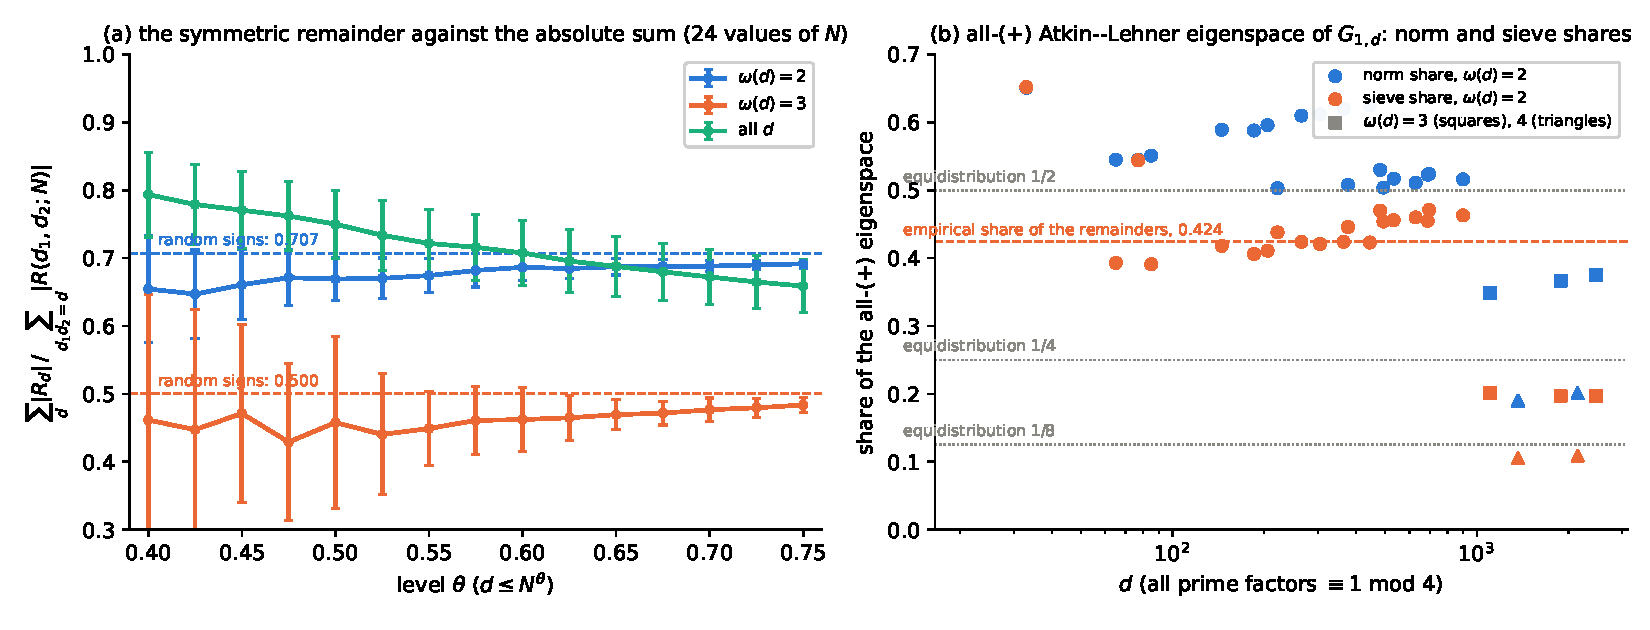
\includegraphics[width=\textwidth]{symmetric_remainder.pdf}
\caption{(a) $\sum_{d\le N^\theta}|R_d|/\sum_{d_1d_2\le N^\theta}|R(d_1,d_2;N)|$ against $\theta$, averaged over $24$ values of $N\approx2\cdot10^6$ (error bars: standard deviation over $N$), for the moduli with two and three prime factors and for all moduli; dashed, the random-sign values $1/\sqrt2$ and $1/2$. (b) The share of the all-$(+)$ joint Atkin--Lehner eigenspace in $G_{1,d}$ for moduli with all prime factors $\equiv1\pmod4$: the Rankin--Selberg norm share (blue) and the share of the sieve coefficients $a(2n')-a(n')$ (orange); circles $\omega(d)=2$, squares $3$, triangles $4$; dotted, the equidistribution values $1/2$, $1/4$, $1/8$; dashed, the empirical share $0.424$ of the remainders. Scripts \texttt{plot\_symmetric\_remainder.py}, \texttt{symmetric\_remainder.py}, \texttt{symmetric\_norm\_share.py}; floating point.}
\label{fig:sym}
\end{figure}

\subsection{Consequence for the sieve}
{\emergencystretch=4em
Corollary~\ref{cor:Rd} replaces, in the remainder sum $2\sum_{m\mid P(z),\,m<y}4^{\omega(m)}|R_m|$ of the two-dimensional sieve (Part~II, (20)), the bound $|R_m|\le\sum_{d_1d_2=m}|R(d_1,d_2)|$ by $2^{\omega(m)}\sum_{t,t_1,s}|c\,a_{P^+G}(N')|$ with $\|P^+G\|\le\|G\|$, and the numerics say that in mean square the gain is the factor $(\text{share})^{1/2}\approx2^{-(\omega(m)-1)/2}$ against the trivial $2^{\omega(m)-1}$ terms: the algebraic cancellation realises the square-root cancellation among the $2^{\omega(m)-1}$ terms that one would expect from independent signs, and essentially nothing beyond it, because the eigenspaces share the norm almost equally. Since $2^{\omega(m)}=m^{o(1)}$, this is absorbed by the factor $N^\eta$ of condition (F1) in the proof of Part~I, Theorem~3.2, and does not change the level of distribution; it changes neither $(7,5)$ nor the constant $0.25$ of Part~II, Theorem~7.1 (the constant is governed by the main term, not by the remainder). The exact identity is nevertheless worth recording: it says that the two-dimensional sieve for $n(N-n)$ sees, at each modulus $d$, only the $W_p$-invariant part of $G_{t,d}$, and therefore none of the oldforms of odd level.
\par}

\section{The dispersion form of the remainder sum and the fixed-argument obstacle}\label{sec:dispersion}

\subsection{The circle modulo $c$}
\begin{lemma}\label{lem:circle}
Let $c$ be odd, $(a,c)=1$ and $h=(h_1,h_2)\in\Z^2$. For odd $c'$ let $c'^{*}$ be the product of the primes dividing $c'$ to an odd power (so $c'^{*}=c'$ for square-free $c'$ and $c'/c'^{*}$ is a square). Then
\[
F_c(a;h):=\sum_{\substack{x,y\bmod c\\ x^2+y^2\equiv a\ (c)}}e\Bigl(\frac{h_1x+h_2y}{c}\Bigr)=\sum_{g\mid(c,h_1,h_2)}g\,\chi\Bigl(\Bigl(\frac cg\Bigr)^{*}\Bigr)\,S\Bigl(a,\ \overline4\,\frac{h_1^2+h_2^2}{g^2};\ \frac cg\Bigr),
\]
with $S(m,n;c)=\sum_{t\bmod c}^{*}e((mt+n\bar t)/c)$ the classical Kloosterman sum ($S(\cdot;1)=1$). For prime $c$ this reads $F_c(a;h)=\chi(c)S(a,\overline4|h|^2;c)+c\,[h\equiv0\ (c)]$.
\end{lemma}
\begin{proof}
Detect the congruence by $\frac1c\sum_{t\bmod c}e(t(x^2+y^2-a)/c)$. For $(t,c)=g$, $t=gt'$, the sum $\sum_{x\bmod c}e((tx^2+h_1x)/c)$ vanishes unless $g\mid h_1$ (shift $x$ by $c/g$), and then equals $g\,e(-\overline{4t'}(h_1/g)^2/(c/g))\,G(t';c/g)$ by completing the square ($2t'$ is invertible modulo $c/g$), where $G(t';c')=\sum_{x\bmod c'}e(t'x^2/c')$. For a prime power, $G(t';p^\nu)=p^{\nu/2}$ if $\nu$ is even and $p^{(\nu-1)/2}(t'/p)\varepsilon_p\sqrt p$ if $\nu$ is odd, with $\varepsilon_p^2=\chi(p)$; by the Chinese remainder theorem $G(t';c')^2=\chi(c'^{*})c'$ for every odd $c'$ (the twisting Jacobi symbols of the reduction square to $1$). Hence
\begin{multline*}
F_c(a;h)=\sum_{g\mid(c,h)}\frac{g^2}{c}\cdot\chi\Bigl(\Bigl(\frac cg\Bigr)^{*}\Bigr)\frac cg\sum_{t'\bmod c/g}^{*}e\Bigl(\frac{-t'a-\overline{4t'}|h/g|^2}{c/g}\Bigr)\\
=\sum_{g\mid(c,h)}g\,\chi\Bigl(\Bigl(\frac cg\Bigr)^{*}\Bigr)S\Bigl(a,\overline4|h/g|^2;\frac cg\Bigr),
\end{multline*}
using $S(-m,-n;c')=S(m,n;c')$. The script \texttt{kloosterman\_check.py} verifies the identity for all $a$, $h$ and all odd primes $c\le61$, for nine square-free composite $c\le105$, and for eleven odd $c\le135$ with square factors (\texttt{results/kloosterman\_check.txt}).
\end{proof}

The general modulus matters below, because the moduli $m'k$ that occur have $k$ an arbitrary divisor of $\beta$, not necessarily square-free. So the Fourier transform of the circle $x^2+y^2\equiv a$ modulo $c$ is a \emph{classical} Kloosterman sum whose second argument is the norm $|h|^2$ of the dual variable, twisted only by a sign; no Sali\'e sum and no character sum of a different type occurs. This is the arithmetic reason why $r(n)$ in arithmetic progressions behaves like the divisor function: the Weil bound gives the asymptotic for $\sum_{n\equiv a\,(c),\,n\le Y}r(n)$ for $c\le Y^{2/3-\e}$, exactly as for $\tau(n)$.

\subsection{The remainder as a trilinear form in Kloosterman sums}\label{subsec:trilinear}
Let $m\equiv m'\equiv1\pmod4$ be coprime, $(mm',N)=1$, $N\equiv2\pmod4$, and let $T^{\mathrm{odd}}(m,m';N)$ be the part of $T(m,m';N)$ with $\alpha$ odd, so that $a_G(N)-a_G(N/2)=T^{\mathrm{odd}}-M^{\mathrm{odd}}$ in \eqref{eq:Rdecomp}. In $T^{\mathrm{odd}}$ every term with $r(\alpha)r(\beta)\ne0$ has $\alpha\equiv\beta\equiv1\pmod4$, so $x^2+y^2=\alpha$ has $x+y$ odd, and $r(\beta)=8\sum_{k\mid\beta,\,k<\sqrt\beta}\chi(k)+4\chi(\sqrt\beta)[\beta=\square]$ by the symmetry $k\leftrightarrow\beta/k$ ($\chi(\beta/k)=\chi(k)$ for $\beta\equiv1\pmod 4$). Writing $\beta=(N-m\alpha)/m'$ and noting that $(k,m)=1$ automatically (a common prime would divide $N$),
\begin{gather}
T^{\mathrm{odd}}(m,m';N)=8\sum_{k<\sqrt{N/m'}}\chi(k)\,\mathcal N_k+4\sum_{j\ge1}\chi(j)\,r^{\mathrm{odd}}\Bigl(\frac{N-m'j^2}{m}\Bigr),\label{eq:Todd}\\
\mathcal N_k=\#\bigl\{(x,y)\in\Z^2:\ x+y\text{ odd},\ x^2+y^2\equiv N\bar m\ (m'k),\ 0<x^2+y^2<Y_k:=(N-m'k^2)/m\bigr\},\notag
\end{gather}
where $r^{\mathrm{odd}}(\alpha)=r(\alpha)[\alpha\text{ odd}]$ and the second sum runs over $j$ with $m\mid N-m'j^2$; it is the number of representations of $N$ by the ternary form $m(x^2+y^2)+m'j^2$ with a sign, and is $O(N^{1/2+\e}m'^{-1/2})$ trivially.

For the lattice-point count $\mathcal N_k$ (with a smooth cutoff $w$ at $Y_k$, the usual sharp-to-smooth passage costing a boundary term), Poisson summation on the residue classes modulo $2c$, $c=m'k$, gives
\begin{equation}\label{eq:poisson}
\mathcal N_k=\frac{Y_k}{2c^2}\sum_{\substack{h\in\Z^2\\ h_1\equiv h_2\ (2)}}\hat w\bigl(h\sqrt{Y_k}/(2c)\bigr)\,F_c\bigl(N\bar m;\ \bar2h\bigr),
\end{equation}
the factor $2[h_1\equiv h_2]$ (absorbed in $1/(2c^2)=2/(2c)^2$) being the Fourier transform of the parity condition and $\bar2h$ the Chinese-remainder twist. The term $h=0$ is $\frac{Y_k}{2c^2}\rho(N\bar m;c)$ with $\rho(a;c)=\#\{x^2+y^2\equiv a\ (c)\}=c\prod_{p\mid c}(1-\chi(p)/p)$, and the sum over $k$ of these terms is the Siegel main term $M^{\mathrm{odd}}(m,m';N)$ (the singular series of the quaternary form, written through the divisor structure of $r(\beta)$). By Lemma~\ref{lem:circle}, for the leading term $g=1$, $\chi(k)\cdot\chi((m'k)^{*})=\chi(k)\chi(k^{*})=\chi(k/k^{*})=1$, since $m'$ is square-free and $\equiv1\pmod4$ and $k/k^{*}$ is an odd square, and
\[
S\bigl(N\bar m,\ \overline{16}\,|h|^2;\ m'k\bigr)=S\bigl(\overline{16m}\,N,\ |h|^2;\ m'k\bigr),
\]
since a Kloosterman sum depends on its two arguments only through their product modulo the modulus ($S(a,b;c)=S(1,ab;c)$ for $(a,c)=1$): the inverse of $16m$ modulo $m'k$ cannot be removed, and the integer $N$ enters multiplied by this unit.\footnote{The archived version~1 of this paper (doi:10.5281/zenodo.23826860), and Part~II, Section~8.1, wrote $S(\overline{16m}N,|h|^2;m'k)$ here. This is incorrect: the products of the arguments differ by the factor $(16m)^2$, and the two sums differ (e.g.\ $N=10$, $m=5$, $c=21$, $|h|^2=5$: $-1.110$ against $-4.494$). The formulas of Sections~\ref{subsec:trilinear}--\ref{subsec:bilinear} are corrected accordingly. The Weil, Cauchy--Schwarz and Poisson computations are unaffected, since they only open the sums; the Kuznetsov heuristic of Section~\ref{subsec:subst}(b) of version~1, which needs fixed integer arguments, is withdrawn; and the numerical experiment of Section~\ref{sec:poisson} has been rerun with the correct sums.} The character $\chi(k)$ of the divisor expansion is exactly cancelled by the sign of the Gauss sums. We have proved:

\begin{proposition}\label{prop:dispersion}
With the notation above,
\begin{multline*}
a_G(N)-a_G(N/2)=8\sum_{k<\sqrt{N/m'}}\ \frac{Y_k}{2(m'k)^2}\sum_{\substack{h\ne0\\ h_1\equiv h_2\ (2)}}\hat w\Bigl(\frac{h\sqrt{Y_k}}{2m'k}\Bigr)\\
\times\sum_{g\mid(m'k,h)}g\,\chi\Bigl(\Bigl(\frac{m'k}{g}\Bigr)^{*}\Bigr)\chi(k)\,S\Bigl(N\bar m,\overline{16}\,\Bigl|\frac hg\Bigr|^2;\frac{m'k}g\Bigr)+\Sigma_\square+\Sigma_\partial,
\end{multline*}
where $\Sigma_\square$ is the ternary term of \eqref{eq:Todd} and $\Sigma_\partial$ the smoothing error; the term $g=1$ is
\begin{equation}\label{eq:main}
8\sum_{k<\sqrt{N/m'}}\frac{Y_k}{2(m'k)^2}\sum_{\substack{h\ne0\\ h_1\equiv h_2\ (2)}}\hat w\Bigl(\frac{h\sqrt{Y_k}}{2m'k}\Bigr)S\bigl(\overline{16m}\,N,\ |h|^2;\ m'k\bigr).
\end{equation}
Consequently the remainder sum of the sieve at the level $N^\theta$, after the decomposition \eqref{eq:Rdecomp} (with the sieve weights and the coefficients $c$ collected into $\Lambda_m,\Lambda'_{m'}\ll3^{\omega}$, and with $m\le m'$ by the symmetry $n\leftrightarrow N-n$), has as its leading term, the contribution of \eqref{eq:main}, the trilinear form
\begin{multline}\label{eq:trilinear}
\mathfrak B=\sum_{m'}\Lambda'_{m'}\sum_{c\equiv0\ (m')}\ \sum_{m}\Lambda_m\sum_{j}b_{m,j}(c)\,S(\overline{16m}\,N,\ j;\ c),\\
b_{m,j}(c)=\frac{4Y_{c/m'}}{c^2}\sum_{|h|^2=j}\hat w\Bigl(\frac{h\sqrt{Y_{c/m'}}}{2c}\Bigr),
\end{multline}
with the modulus $c=m'k$ in the progression $c\equiv0\pmod{m'}$, $c\le\sqrt{Nm'}$, the first argument $\overline{16m}N$, the fixed integer $N$ multiplied by the inverse of $16m$ modulo the modulus, the second argument $j=|h|^2$ a norm, and smooth weights in $c$ and $h$.
\end{proposition}

\begin{remark}\label{rem:disp}
(i) The dual variable satisfies $|h|\ll m'k\sqrt{m/N}\,N^\e$; so the inner sum of \eqref{eq:main} is empty unless $k\gg\sqrt{N/m}/m'$, the modulus runs in $\sqrt{N/m}\ll c\le\sqrt{Nm'}$, and $j=|h|^2\ll mm'^2k^2/N\le mm'$. The sum over $k$ has length $K\asymp\sqrt{N/m'}$.

(ii) Opening the Kloosterman sum, \eqref{eq:main} is the Kloosterman refinement of the circle method for the quaternary form $Q_{m,m'}$, with the moduli $m'k$ ordered by the divisor structure of $r(\beta)$. The sum over $k$ is, however, not of the form $\sum_{c\equiv0\,(m')}S(a,b;c)\phi(c)/c$ with integers $a,b$ independent of $c$, to which the Kuznetsov formula for $\Gamma_0(m')$ applies: the first argument $\overline{16m}N$ is a residue class modulo $c$, and its integer representatives $(N+tc)/(16m)$, $t\equiv-N\bar c\pmod{16m}$, vary with $c$ even within a class of $c$ modulo $16m$ (the class $t=0$ is empty, as $16\nmid N$). The spectral form of the sum over the moduli would therefore involve Kloosterman sums with a modulus-dependent argument, and we do not know how to write it through the Fourier coefficients of the Maass forms of level $m'$ in a useful way. What the theta function does is to evaluate the sum over $k$ at the level $4mm'$ of the quaternary form, where $k$ is the index of a Fourier coefficient and not a modulus (Section~\ref{subsec:subst}).

(iii) This is the two-sided version of Linnik's problem $N=p+x^2+y^2$, for which the dispersion method was invented \cite{Linnik}: there $\sum_pr(N-p)=4\sum_p\sum_{k\mid N-p}\chi(k)$ is a Titchmarsh-type sum with the moduli $k$ up to $N$ and the primes as the rough variable. Here both sides carry $r$, both carry sieve weights, and the divisor structure of one side ($\beta$) provides the moduli $m'k$ while the lattice structure of the other side ($\alpha=x^2+y^2$) provides the Kloosterman sums.

(iv) \emph{What is left aside.} The terms with $g>1$ in Proposition~\ref{prop:dispersion} are sums of the same shape with the modulus $m'k/g$ and the dual variable $h/g$, $g\mid(m'k,h_1,h_2)$, with fewer terms; the ternary term $\Sigma_\square\ll N^{1/2+\e}m'^{-1/2}$ sums over $mm'\le N^\theta$ to $\ll N^{1/2+3\theta/4+\e}$, harmless for $\theta<2/3$; and $\Sigma_\partial$ is the usual price of a smooth cutoff at $Y_k$ (a dyadic decomposition with $\hat w(\xi)\ll(1+|\xi|)^{-A}$). We have not carried these bookkeeping steps out in detail: the exponent analysis of Sections~\ref{subsec:book}--\ref{subsec:subst} and \ref{sec:poisson} concerns the leading term \eqref{eq:main}, and \eqref{eq:trilinear} is the form of the remainder sum in this sense.
\end{remark}

\subsection{Exponent bookkeeping}\label{subsec:book}
In \eqref{eq:main}, for each $k$ the number of $h$ is $\asymp(m'k)^2m/N$ and the weight $Y_k/(2(m'k)^2)\asymp N/(m(m'k)^2)$, so each $k$ contributes $O(1)$ terms of weight $O(1)$ on average.
\begin{itemize}[leftmargin=1.6em]
\item \emph{Weil bound only.} $|S(\overline{16m}N,|h|^2;c)|\le d(c)c^{1/2}(|h|^2,c)^{1/2}$ gives $|a_G(N)-a_G(N/2)|\ll N^\e\sum_{k\le\sqrt{N/m'}}(m'k)^{1/2}\ll N^{3/4+\e}m'^{-1/4}$, and the sum of absolute values over $mm'\le N^\theta$ is $\ll N^{3/4+\theta+\e}$: level $1/4$.
\item \emph{The theta-function bound.} Theorem~1.1(ii) of Part~II (Theorem~2.3 of Part~I), $|a_G(N)|\ll N^{1/2+\e}$, is smaller than the Weil bound by exactly $(N/m')^{1/4}=K^{1/2}$: it is equivalent to square-root cancellation in the sum over the moduli $c=m'k\equiv0\pmod{m'}$, $k\le K$, for the specific arguments $\overline{16m}N$ and $|h|^2$. Summing absolute values over $mm'\le N^\theta$ gives the level $1/2$ (Part~I, Theorem~3.2).
\item \emph{Cancellation over $m'$.} If $\sum_{m'\sim E}\Lambda'_{m'}\bigl(a_{G_{m,m'}}(N)-a_{G_{m,m'}}(N/2)\bigr)\ll N^{1/2+\e}E^{1/2}$ for each $m\le\Delta$ (square-root cancellation among the $E$ values of $m'$), the remainder is $\ll N^{1/2+\e}\Delta E^{1/2}$, which is $\ll N^{1-\delta}$ for $\Delta^2E\le N^{1-3\delta}$; with the balanced split $\Delta=E=N^{\theta/2}$ (the hardest case, which the sieve needs) this is $\theta<2/3$. The same conclusion follows from Part~II, Proposition~4.2, with a saving $E^{-1/2}$ in place of $(de)^{-\eta}$.
\item \emph{Cancellation over $m'$ and $m$.} Square-root cancellation over both gives $N^{1/2+\e}(\Delta E)^{1/2}$ and the level $1-\e$.
\end{itemize}
The data of Part~II, Section~8.2 (the signed sums over $(d,e)$ are of the size of the root mean square, for all three weightings and all $\theta\le3/4$) are consistent with the last two items; they say nothing about a proof.

\subsection{What the dispersion method must deliver, and what is available}\label{subsec:deliver}
The form \eqref{eq:trilinear} is the type of sum treated by Deshouillers and Iwaniec \cite[Theorems~9--12]{DI}, bilinear forms $\sum_{c\equiv0\,(q)}\sum_m\sum_na_mb_ng(c,m,n)S(m,\pm n;c)$ bounded through the Kuznetsov formula and the spectral large sieve, and by Drappeau's extension \cite[Theorem~2.1]{Drappeau} with a congruence condition on the modulus: in his normalisation, for $b_{n,r,s}$ supported on $n\le N_0$, $r\sim R$, $s\sim S$, moduli $sc$ with $c\sim C$ in a class modulo $q$ and $d\sim D$ in a class modulo $q$,
\begin{gather*}
\sum\sum b_{n,r,s}\,g(c,d,n,r,s)\,e\Bigl(\frac{n\,\overline{rd}}{sc}\Bigr)\ll(qCDN_0RS)^{\e}\,q^{3/2}K\,\|b\|_2,\\
K^2=qCS(RS+N_0)(C+RD)+C^2DS\sqrt{(RS+N_0)R}+D^2N_0R/S .
\end{gather*}
To apply such a bound to \eqref{eq:trilinear} one has to overcome three specific features.
\begin{enumerate}[label=\textup{(\alph*)},leftmargin=2.2em]
\item \emph{The first argument is fixed, and carries a unit.} In \eqref{eq:trilinear} there is no average over the first argument $\overline{16m}N$: it is the single integer $N\gg c$, multiplied by the inverse of $16m$ modulo the modulus, whereas the known applications (BFI \cite{BFI}, the Titchmarsh divisor problem) average over a long variable in both arguments. The unit $\overline{16m}$ depends on the modulus, so that the sum over $c$ is not of the form $\sum_cS(a,b;c)\phi(c)$ with fixed $a,b$ to which the Kuznetsov formula applies (Remark~\ref{rem:disp}(ii)); and the one-sided average that is available is over the norms $j=|h|^2\le mm'$ with the coefficient $r(j)\cdot(\text{weights})$, of length $\ll\Delta E$, the variable $m$ sitting in the unit.
\item \emph{The sieve weight sits on the divisibility class of the modulus.} The sum over $m'$ in \eqref{eq:trilinear} is over the \emph{class} $c\equiv0\pmod{m'}$ with the weight $\Lambda'_{m'}$. This is where BFI use the well-factorable structure of the linear sieve weights, $\Lambda'=\Lambda'_1*\Lambda'_2$ with $m'=m'_1m'_2$ in prescribed ranges, so that the modulus $c=m'_1m'_2k$ has two smooth factors; the weights of the two-dimensional sieve (DHR) are not well-factorable in Iwaniec's sense, and one would first have to go back to a vector or $\beta$-sieve with well-factorable weights, at the price of $(7,5)$.
\item \emph{The hard range.} The Kloosterman regime is $c\in[\sqrt{N/m},\sqrt{Nm'}]$, always beyond $\sqrt N$; and since the first argument $\overline{16m}N$ depends on the modulus (Remark~\ref{rem:disp}(ii)), there is no fixed Bessel argument $4\pi\sqrt{ab}/c$ and no Kuznetsov transform in the usual sense. With the representatives $(N+tc)/(16m)$ the argument $4\pi\sqrt{(N+tc)j/(16m)}/c$ is of constant size in $k$ throughout the range of the sieve, so that even class by class the transform would not localise the spectrum.
\end{enumerate}
We have not carried out the estimation, and we make no claim of a level $>1/2$. What the computation establishes is the exact shape of the problem: after the theta-function saving (the sum over $k$), the remainder sum is $N^{1/2+\e}\sum_{m\le m'}|\Lambda_m\Lambda'_{m'}|$, and any power saving in the sum over the sieve modulus $m'$ of the Kloosterman sums \eqref{eq:main}, uniform in $m\le m'$, raises the level beyond $1/2$ (Part~II, Proposition~4.2); the heuristic ceiling of the method, square-root cancellation over $m'$, is the level $2/3$, which would give $(6,4)$ for every $N$ (Part~II, Table~4). Whether the specific levels $4/7$ or $13/25$ are attainable is open.

\subsection{Substituting the Deshouillers--Iwaniec bounds: where the exponent is lost}\label{subsec:subst}
We now carry out the substitution of the available bounds into \eqref{eq:trilinear} explicitly, in order to name the term that blocks $\theta>1/2$. Throughout $m\asymp\Delta$, $m'\asymp E$, $k\asymp K=\sqrt{N/E}$, $c=m'k\asymp C_0:=\sqrt{NE}$, the second argument $n=mj$ runs up to $\mathcal N:=\Delta H^2\asymp\Delta^2E$ with $\|b\|_2^2\asymp\mathcal N^{1+o(1)}$, the weight of one term is $\asymp N/(mC_0^2)=1/(\Delta E)$, and the target for the $m$-th piece $\mathfrak B_m$ is $N^{1-\delta}/\Delta$. Two reference points: the Weil bound gives $\sum_{m'}|\cdot|\ll E\cdot N^{3/4}E^{-1/4}$ (Section~\ref{subsec:book}), and the theta-function bound gives $EN^{1/2+\e}$.

\emph{(a) Drappeau's Theorem~2.1.} The sum there is $\sum_{c,d,n,r,s}b_{n,r,s}g(c,d,n,r,s)e(n\overline{rd}/(sc))$, with $c\equiv c_0$, $d\equiv d_0\pmod q$, $g$ smooth with $\partial_d^\nu g\ll d^{-\nu(1-\e_0)}$, and the Kloosterman fraction comes from an \emph{incomplete} sum over the inverse variable $rd$ of a \emph{linear} congruence. Neither feature is present in \eqref{eq:trilinear}: the congruence $x^2+y^2\equiv N\bar m\pmod{m'k}$ is quadratic, and the Gauss-sum evaluation of Lemma~\ref{lem:circle} has already completed the sum over the inverse variable, producing $S(\overline{16m}N,j;c)=\sum_{t\bmod c}^*e(\overline{16m}Nt/c)e(j\bar t/c)=\sum_{s\bmod c}^*e(Ns/c)e(\overline{16m}j\bar s/c)$. To write this in Drappeau's form one has to let the inverse variable run over a full period, with $s=m'$ ($S=E$), his $c=k$ ($C=K$), $r=16m$ ($R=16\Delta$: the unit $\overline{16m}$ is his $\bar r$), $D=EK$, $q=1$, and then either
\begin{itemize}[leftmargin=1.6em]
\item[I.] $n=N$ (a single value, $N_0=N$, $\|b\|_2=1$, the inverse variable being $\bar s$) and the factor $e(js/c)$ pushed into $g$, which violates the smoothness hypothesis because its frequency $j/c$ is not $\ll1/D$; or
\item[II.] $n=j$ ($N_0=\Delta E$, the inverse variable being $t$) and the factor $e(\overline{16m}Nt/c)$ pushed into $g$, which violates it even more violently.
\end{itemize}
Formally, i.e.\ ignoring the violated hypothesis, with $R=16\Delta$ the three terms of $K^2=qCS(RS+N_0)(C+RD)+C^2DS\sqrt{(RS+N_0)R}+D^2N_0R/S$ are, in case~I, $\asymp K^2E^2\Delta N$, $K^3E^2(\Delta N)^{1/2}$ and $K^2E\Delta N$, so that $K\asymp KE(\Delta N)^{1/2}$ and the bound for one $j$ is $\asymp N(\Delta E)^{1/2}$; after the normalisation $1/(\Delta E)$ and the sum over the $\asymp\Delta E$ values of $j$ this is $\gg N(\Delta E)^{1/2}$, worse than the trivial bound. The culprit is the single numerator $N$, in the first and in the third term. In case~II the terms are $\asymp K^2E^3\Delta^2$, $K^3E^{5/2}\Delta$ and $E^2K^2\Delta^2$, the first dominates, $K\asymp KE^{3/2}\Delta$, and $|\mathfrak B_m|\ll N^{1/2}E^{1/2}\Delta^{1/2}N^{\e}$ after the normalisation and the sum over $j$; the target $N^{1-\delta}/\Delta$ then needs $\Delta^{3/2}E^{1/2}\le N^{1/2}$, i.e.\ $\Delta E\le N^{1/2}$ for the balanced split: exactly the level $1/2$ of the theta-function bound, and not more, for the same reason as in (A1) of Section~\ref{subsec:CS} (the term $qCS\cdot N_0\cdot RD$ is the diagonal of a Cauchy--Schwarz over the short variables). So even formally neither assignment goes beyond $1/2$.

\emph{(b) The Kuznetsov route.} The results of \cite{DI} that apply to complete Kloosterman sums with $c\equiv0\pmod q$ go through the Kuznetsov formula for $\Gamma_0(q)$, which requires the two arguments to be integers independent of the modulus. In \eqref{eq:trilinear} the first argument is $\overline{16m}N$, a residue class modulo $c$ whose integer representatives vary with $c$ (Remark~\ref{rem:disp}(ii)), so the sum over $c\equiv0\pmod{m'}$ is not a sum $\sum_cS(a,b;c)\phi(c)/c$ with fixed $a,b$, and the Kuznetsov formula does not apply to it as it stands. (Version~1 of this paper applied it with the arguments $16N$ and $mj$, on the strength of the incorrect identity corrected in Section~\ref{subsec:trilinear}; that computation, which concluded that the route reproduces the Weil bound, is withdrawn.) We do not know a spectral expansion adapted to a modulus-dependent unit in one argument. The theta function evaluates the sum over $k$ at the level $4mm'$ of the quaternary form, where $k$ is the index of a Fourier coefficient and not a modulus, and this is why it reaches $N^{1/2}$: there is no argument to average.

\emph{Conclusion of the substitution.} In every assignment, the quantity that blocks $\theta>1/2$ is the single large argument $N$, carried by the unit $\overline{16m}$ modulo the modulus: as the numerator $N_0=N$ in Drappeau's bound (case~I), as the diagonal term $qCS\cdot N_0\cdot RD$ (case~II), and as the obstacle to any spectral expansion. A proof of a level beyond $1/2$ along these lines would have to average over $N$ (which is Theorem~1.3 of Part~II, the almost-all-$N$ result, and Section~\ref{sec:short} below) or exploit the specific structure of the arguments, $N$ against the norms $j=|h|^2$ and the unit $\overline{16m}$, which is not a feature the general bounds see.

\section{Cauchy--Schwarz and Poisson duality against the fixed first argument}\label{sec:poisson}

The obstacle (a) of Section~\ref{subsec:deliver} is that the first argument $\overline{16m}N$ of the Kloosterman sums in \eqref{eq:trilinear} is not averaged. Here we examine whether it can be dualised away: fix $m\asymp\Delta$, apply Cauchy--Schwarz over the smooth variables, expand the square over $m'_1,m'_2\asymp E$, and apply Poisson summation to $h\in\Z^2$. The outcome is negative, for a reason that is worth stating precisely: in \eqref{eq:trilinear} the box of $h$ has side $H\le\sqrt{mm'}$, while the modulus of the Poisson step is at least $\sqrt N$; the dual of a short sum is a long sum.

\subsection{The sizes}
Fix $m\asymp\Delta$ and dyadic $m'\asymp E$, $k\asymp K\le\sqrt{N/E}$, and put $c=m'k$. In \eqref{eq:main} the weight is $\asymp W_0:=N/(mE^2K^2)$ and $\hat w$ localises $h$ to $|h|\le H:=EK\sqrt{m/N}$, so that
\begin{equation}\label{eq:sizes}
H^2=\frac{E^2K^2m}{N}\le mE=mm',\qquad H^2W_0\asymp1,\qquad \#\{(k,h)\}\asymp KH^2 .
\end{equation}
The Kloosterman regime is $K\ge\sqrt{N/m}/E$ (Remark~\ref{rem:disp}(i)), and the top range $K\asymp\sqrt{N/E}$, where $H^2\asymp mm'$, dominates.

\subsection{Two Cauchy--Schwarz arrangements}\label{subsec:CS}
Let $\mathfrak B_m=\sum_{m'}\Lambda'_{m'}\sum_k\sum_hw\,S(\overline{16m}N,|h|^2;m'k)$ be the $m$-th piece of \eqref{eq:trilinear}; the target is $|\mathfrak B_m|\le N^{1-\delta}/\Delta$, and the theta-function bound gives $|\mathfrak B_m|\ll EN^{1/2+\e}$.

\emph{(A1) Smooth variables outside, $m'$ inside.} By Cauchy--Schwarz over $(k,h)$,
\begin{multline*}
|\mathfrak B_m|^2\le\Bigl(\sum_{k,h}W_0^2\Bigr)\sum_{k,h}\Bigl|\sum_{m'}\Lambda'_{m'}S(\overline{16m}N,|h|^2;m'k)\Bigr|^2\\
\asymp\frac{N}{mE^2K}\Bigl(\sum_{m'}\sum_{k,h}|S(\overline{16m}N,|h|^2;m'k)|^2+\text{off-diagonal}\Bigr).
\end{multline*}
The diagonal is the mean square of Kloosterman sums over $h$, which is $\asymp H^2c$ by Weil (and is sharp: the mean of $|S(a,n;c)|^2$ over $n$ is $\varphi(c)$), so it contributes $E\cdot K\cdot H^2\cdot EK=E^2K^2H^2$ and
\[
|\mathfrak B_m|^2\ll\frac{N}{mE^2K}\,E^2K^2H^2=E^2K^3,\qquad |\mathfrak B_m|\ll EK^{3/2}=E^{1/4}N^{3/4}\quad(K=\sqrt{N/E}),
\]
\emph{even if the off-diagonal terms vanished}. This beats $EN^{1/2}$ only for $E>N^{1/3}$, and the sieve condition $\Delta E^{1/4}N^{3/4}\le N^{1-\delta}$ with the balanced split $\Delta=E$ gives $E\le N^{1/5}$, i.e.\ the level $2/5<1/2$. The diagonal already loses, because Cauchy--Schwarz replaces the theta-function saving $K^{1/2}$ on the sum over $k$ by the Weil bound: the smooth variables are too short to carry the dispersion.

\emph{(A2) $h$ outside, $(m',k)$ inside.} Now $|\mathfrak B_m|^2\le(\sum_hW_0^2)\sum_h|\sum_{m',k}S|^2$, the diagonal is $H^2\cdot EK\cdot EK$, and with \eqref{eq:sizes}
\[
|\mathfrak B_m|^2\ll H^2W_0^2\cdot H^2E^2K^2=E^2K^2,\qquad|\mathfrak B_m|\ll EK=\sqrt{EN},
\]
which is the level-$2/3$ target of Section~\ref{subsec:book}; but this diagonal \emph{is} the statement that the sum over the moduli $c=m'k$ has square-root cancellation, so (A2) is a reformulation of the problem, not a method, and everything is in the off-diagonal terms
\begin{equation}\label{eq:corr}
C(c_1,c_2)=\sum_hW\Bigl(\frac hH\Bigr)S(\overline{16m}N,|h|^2;c_1)\,S(\overline{16m}N,|h|^2;c_2),\qquad c_i=m'_ik_i,\ c_1\ne c_2 ,
\end{equation}

the inverse of $16m$ being taken modulo $c_1$ in the first factor and modulo $c_2$ in the second.

\subsection{Poisson in $h$ for the off-diagonal terms}
Opening the two Kloosterman sums in \eqref{eq:corr}, with the substitutions $t_i\mapsto16mt_i$, $g=(c_1,c_2)$ and $q=[c_1,c_2]=c_1c_2/g$,
\begin{gather*}
C(c_1,c_2)=\sum_{t_1\bmod c_1}^*\sum_{t_2\bmod c_2}^*e\Bigl(\frac{Nt_1}{c_1}+\frac{Nt_2}{c_2}\Bigr)\,\mathcal G(\lambda),\\
\mathcal G(\lambda)=\sum_{h\in\Z^2}W\Bigl(\frac hH\Bigr)e\Bigl(\frac{\lambda|h|^2}{q}\Bigr),\qquad \lambda=\overline{16m}\Bigl(\bar t_1\frac{c_2}g+\bar t_2\frac{c_1}g\Bigr)
\end{gather*}
(the unit $\overline{16m}$ modulo $q$ sits in $\lambda$, where it is harmless: $(\lambda,q)$ and $|G(\lambda;q)|$ do not see it).
The inner sum is a two-dimensional theta sum of length $H$ and modulus $q$. Poisson summation (write $h=u+qv$, $u\bmod q$) gives, for $(\lambda,q)=1$,
\[
\mathcal G(\lambda)=\frac{H^2}{q^2}\sum_{\ell\in\Z^2}\hat W\Bigl(\frac{H\ell}q\Bigr)\sum_{u\bmod q}e\Bigl(\frac{\lambda|u|^2+\ell\cdot u}{q}\Bigr)=\frac{H^2}{q^2}\sum_{\ell\in\Z^2}\hat W\Bigl(\frac{H\ell}q\Bigr)G(\lambda;q)^2\,e\Bigl(-\frac{\overline{4\lambda}\,|\ell|^2}{q}\Bigr),
\]
with $|G(\lambda;q)|^2=q$. The dual variable runs over $|\ell|\ll q/H$, so the dual sum has $(q/H)^2$ terms of size $H^2/q$, and the fixed $N$ survives as the linear phase of the two-variable complete sum
\[
\sum_{t_1,t_2}e\Bigl(\frac{Nt_1}{c_1}+\frac{Nt_2}{c_2}-\frac{\overline{4\lambda(t_1,t_2)}\,|\ell|^2}{q}\Bigr)G(\lambda(t_1,t_2);q)^2 ,
\]
in which $\lambda$ is a linear form in the inverses $\bar t_1,\bar t_2$: this is the ``congruence equation in $(t_1,t_2)$'' that the dualisation produces. Now the bookkeeping. The term $\ell=0$ gives $(H^2/q)\chi(q)$ times a sum of $e(Nt_1/c_1+Nt_2/c_2)$ over $(t_1,t_2)$ with $(\lambda,q)=1$, a combination of Ramanujan sums, hence $O(H^2g\,N^\e/q)$: the off-diagonal has no main term, in agreement with the random-sign behaviour of Part~II, Section~8.2. For $\ell\ne0$, even with square-root cancellation of Deligne type in the $(t_1,t_2)$-sum (which has $c_1c_2=qg$ terms), the total is
\[
\frac{H^2}{q^2}\cdot\Bigl(\frac qH\Bigr)^2\cdot q\cdot(qg)^{1/2}=q^{3/2}g^{1/2},
\]
against the trivial bound $H^2(c_1c_2)^{1/2}=H^2(qg)^{1/2}$ obtained by applying Weil to both Kloosterman sums before summing over $h$. (The terms with $(\lambda,q)>1$, where the Gauss sums degenerate, are left aside, and the square-root cancellation in the $(t_1,t_2)$-sum is an assumption, not a theorem: it would need a non-degeneracy statement for the phase that we have not examined. This is bookkeeping under the most favourable assumption, which is enough for a negative conclusion.) The dualisation therefore loses the factor
\[
\frac q{H^2}\ \ge\ \frac{c_1c_2/g}{mm'}\ \ge\ \frac{\sqrt{EN}}{m}\ \ge\ N^{1/2-\theta/4}\qquad(\text{balanced split }m\asymp m'\asymp N^{\theta/2}),
\]
and it would gain only if $H>\sqrt q$, i.e.\ $mm'\gg\sqrt{EN}$, which never happens for $\theta<2$. By \eqref{eq:sizes} the side of the $h$-box is at most $\sqrt{mm'}=N^{\theta/2}$, the square root of the sieve level, while every modulus in \eqref{eq:trilinear} is at least $\sqrt{N/m}$; Poisson in $h$ is counterproductive in the whole range of the sieve.

\subsection{Conclusion, and what the data say}
Neither Cauchy--Schwarz arrangement removes the fixed first argument: (A1) is weaker than the theta-function bound because it discards the saving on the $k$-sum, (A2) is a restatement, and the Poisson dual of the $h$-sum is longer than the sum itself by $N^{1/2-\theta/4}$. The only variable in \eqref{eq:trilinear} that is long compared with the modulus is $k$, and that is the modulus; its sum is exactly what the theta function already evaluates. A dispersion over the lattice points $(x,y)$ themselves (the arrangement of Linnik's problem, the sum over $m'$ inside the square) leads to the correlations $\sum_{m\alpha+[e_1,e_2]\beta=N}r(\alpha)r(e_1'\beta)r(e_2'\beta)$, whose weight $r(e_1'\beta)r(e_2'\beta)$ is not a theta coefficient and whose moduli $[e_1,e_2]\asymp E^2$ cost, with the theta bound, the level $1/3$; this is where the Deshouillers--Iwaniec machinery would have to enter, and it is the problem of Section~\ref{subsec:deliver}, not a way around it.

The script \texttt{kloosterman\_correlation.py} (\texttt{results/kloosterman\_correlation.txt}) computes \eqref{eq:corr} for $N=2000002$, $m=5$, twelve primes $m'\in[41,173]$ and $k=43,83,127$, i.e.\ moduli $c\le2.2\cdot10^4$ in the Kloosterman regime: there $H$ is between $2.8$ and $35$, $H^2/c^2=m/N=2.5\cdot10^{-6}$ exactly, the diagonal $C(c,c)$ is between $0.3$ and $2.6$ times the Weil size $H^2c$ (median $0.85$; the mean of $|S(a,n;c)|^2$ over $n$ is $\varphi(c)$, and the boxes here hold only $3$ to $600$ points), the off-diagonal correlations $C(c_1,c_2)/\sqrt{C(c_1,c_1)C(c_2,c_2)}$ have root mean square $0.29$, $0.16$, $0.12$ (random signs on the $\asymp H^2$ lattice points would give $0.19$, $0.10$, $0.06$), and the quadratic form $\sum_{m'_1,m'_2}\pm\pm C$ is $0.74$, $1.10$, $0.77$ times its trace for coherent signs and $0.99$--$1.00$ for random signs, against $12$ for full coherence (Figure~\ref{fig:kloost}): square-root cancellation over $m'$, as in Part~II, Section~8.2, and nothing that a dualisation of $h$ could exploit.

\begin{figure}[htbp]
\centering
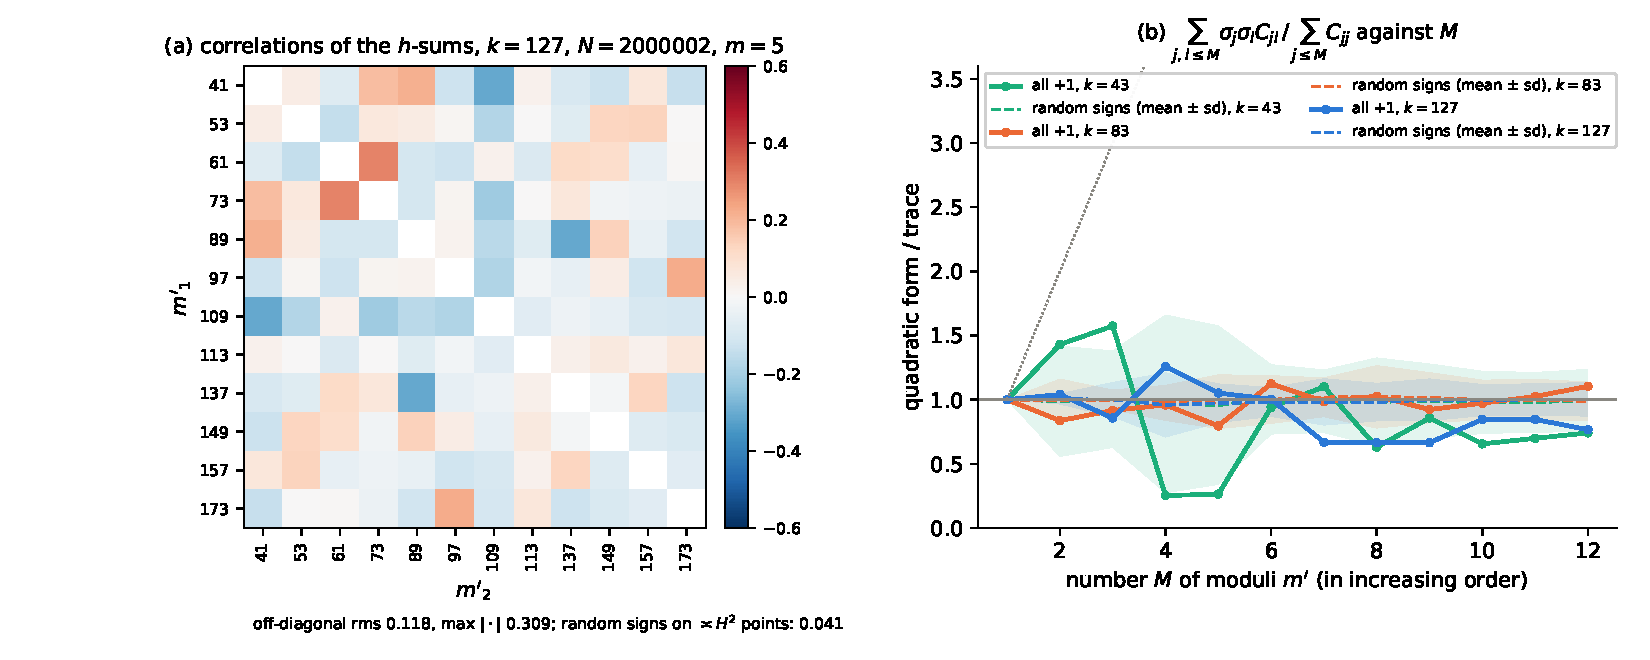
\includegraphics[width=\textwidth]{kloosterman_correlation.pdf}
\caption{(a) The correlation matrix $C(c_1,c_2)/\sqrt{C(c_1,c_1)C(c_2,c_2)}$ of the $h$-sums \eqref{eq:corr} for $N=2000002$, $m=5$, $k=127$ and twelve primes $m'$ (diagonal blanked). (b) The quadratic form $\sum_{j,l\le M}\sigma_j\sigma_lC(m'_jk,m'_lk)$ divided by its trace against the number $M$ of moduli, for coherent signs $\sigma\equiv1$ (solid) and for random signs (dashed, mean and one standard deviation over $200$ draws), for $k=43,83,127$; dotted, full coherence $=M$. Script \texttt{plot\_kloosterman\_correlation.py}; floating point.}
\label{fig:kloost}
\end{figure}

\subsection{The bilinear form in the two moduli}\label{subsec:bilinear}
The factorisation of the modulus $c=m'k$ makes precise where a saving would have to come from. For $(k,m')=1$ (the generic case in \eqref{eq:main}, $m'$ being square-free; the terms with $(k,m')>1$ have fewer $k$) the Chinese remainder theorem factors the Kloosterman sum \cite[(1.59)]{IK}:
\begin{equation}\label{eq:CRT}
S(a,n;m'k)=S(a\bar k,\,n\bar k;\,m')\;S(a\overline{m'},\,n\overline{m'};\,k),\qquad a=\overline{16m}N,\quad n=|h|^2,
\end{equation}
with $k\bar k\equiv1\pmod{m'}$ and $m'\overline{m'}\equiv1\pmod k$, the inverse $\overline{16m}$ in $a$ being taken modulo $m'$ in the first factor and modulo $k$ in the second (by the change of variable $t\mapsto\bar kt$ modulo $m'$ the first factor is also $S(a\bar k^2,n;m')$, the form in which the factorisation is often written, and likewise the second). The $m$-th piece of \eqref{eq:trilinear} is therefore the bilinear form in the two moduli
\begin{equation}\label{eq:bilinear}
\mathfrak B_m=\sum_{m'}\Lambda'_{m'}\sum_{k\le K}\sum_{h}w_{k,m'}(h)\,S(\overline{16m}N\bar k,|h|^2\bar k;m')\,S(\overline{16m}N\overline{m'},|h|^2\overline{m'};k),
\end{equation}
with the sieve weights $\Lambda'$ on $m'\le E$, smooth weights in $k\asymp K=\sqrt{N/E}$ and $h$, and $|h|\le H\le\sqrt{mm'}$. Three remarks.

(i) \emph{The fixed argument modulo $m'$ is $\overline{16m}N\bar k$.} As $k$ runs over its range of length $K\ge m'$ (for $m'\le N^{1/3}$, i.e.\ throughout the sieve range $E\le N^{\theta/2}$, $\theta\le2/3$), the class $\bar k\pmod{m'}$ runs through every reduced class about $K/m'$ times: modulo $m'$ the first argument is equidistributed over $k$. This mixing is real, and it is already fully used: the sum over $k$ at fixed $m'$ with the theta-function bound is the square-root cancellation of Section~\ref{subsec:book}, and no arrangement of the $k$-sum alone gives more (Section~\ref{subsec:CS}, (A2)). A saving beyond the theta bound must come from the interaction of the two moduli.

(ii) \emph{What is required is a bilinear estimate.} In \eqref{eq:bilinear} the second factor has modulus $k\asymp\sqrt{N/E}\ge\sqrt N/E$ and depends on $m'$ through $\bar m'\pmod k$ and through the weight; the $h$-sum is short relative to both moduli (Section~\ref{subsec:CS}) and does not complete to a Gauss sum, which is why Poisson in $h$ fails. The statement that would give a level beyond $1/2$ is a bound $\mathfrak B_m\ll E^{1/2-\delta}N^{1/2+\e}$ for arbitrary bounded $\Lambda'$ (Part~II, Proposition~4.2 converts any $\delta>0$ into a level beyond $1/2$), uniformly in the single fixed $N$. This is the shape of the bilinear forms in Kloosterman-type sums with a fixed numerator and moduli in a bilinear range that occur in the equidistribution of roots of quadratic congruences (Duke--Friedlander--Iwaniec \cite{DFI}, Fouvry--Iwaniec \cite{FI}; Lemma~\ref{lem:circle} exhibits the present sums as the two-variable analogue, the circle $x^2+y^2\equiv16N\pmod{m'k}$), where the saving comes from the spectral theory of the Weyl sums over the roots and not from Weil's bound. Whether that theory applies with the sieve weights on $m'$ and the theta-type weight in $h$ is the precise form of the open question of Section~\ref{subsec:deliver}.

(iii) \emph{The diagnosis is sharpened, not changed.} The obstruction ``fixed $16N$'' of Sections~\ref{subsec:subst} and \ref{sec:poisson} is, in \eqref{eq:bilinear}, the absence of an independent average over the first arguments; the factorisation shows what replaces it, the joint variation of $(\bar k\bmod m',\ \bar m'\bmod k)$, and that any saving must be bilinear, as in \cite{BFI,DFI}. The data of this section measure the $m'$-side of the interaction at fixed $k$ (the correlations $C(c_1,c_2)$ with $c_i=m'_ik$) and find square-root cancellation; the $k$-side at fixed $m'$ is the theta bound; the open question is whether the two savings can be combined.

\section{The dimension of the weighted sieve and mollified theta weights}\label{sec:dimension}

\subsection{Where $2^{\Omega}$ enters}\label{subsec:omega}
The weighted sieve of Part~II, Section~7.2, gives $W\ge X_NV(z)(L_2-\lambda R_2-o(1))$ for
\[
W=\sum_{\substack{n\in\cA\\ (n(N-n),P(z))=1}}w(n)\Bigl(1-\lambda\sum_{\substack{z\le p<y\\ p\mid n(N-n)}}\Bigl(1-\frac{\log p}{\log y}\Bigr)\Bigr),
\]
and the count of integers follows from $w(n)=16\cdot2^{\Omega(n(N-n))}\le2^{k+4}$ on the integers with positive weight. The pairs $(k,k')$ are decided by the inequalities $1/\lambda+2/b\le k+1$ and $1/\lambda+1/b\le k'+1$ together with $L_2-\lambda R_2>0$; the factor $2^{\Omega}$ enters only in the final division by $\max w$, i.e.\ in the constant $0.25$ of Theorem~7.1 and nowhere else. Removing it would improve the constant by at most $2^{k+4}$ and would not change $(k,k')$. The Buchstab identity does not help here either: $W$ is a sum of non-negative weights $w(n)\cdot(\text{Richert weight})$, and writing $w(n)=2^{j}\cdot16$ on $\{\Omega(n(N-n))=j\}$ one has $\#\{n\}\ge\sum_jW_j\ge W/2^{k+4}$ with $W_j\ge0$; without a lower bound for the individual $W_j$, which the sieve does not provide, the division by $2^{k+4}$ is the best possible.

\subsection{The dimension}\label{subsec:dim}
What the weights $r(n)r(N-n)$ really cost is the dimension. Under $w$, the density of $p\mid n(N-n)$ on $\cA$ is $2h(p)\sim4/p$ for split $p$ and $2h(q)\sim2/q^2$ for inert $q$, so $\sum_{p<z}\omega(p)/p=2\log\log z+O(1)$: dimension $\kappa=2$. Under the indicator weight $b(n)b(N-n)$ ($n$ and $N-n$ sums of two squares) the density of $p\mid n$ among the sums of two squares is $\sim1/p$ for split $p$ (since $n=pn'$ is a sum of two squares iff $n'$ is) and $\sim1/q^2$ for inert $q$, so the two sides together have $\sum_{p<z}\omega(p)/p=\log\log z+O(1)$: dimension $\kappa=1$, the dimension of Goldbach's problem. The factor $2$ in $r(pn')=2r(n')$ is this doubling of the density, not a weight attached to the sifted integers that could be dropped.

The script \texttt{dimension\_benchmark.py} computes, with the sieve functions of Part~II (\texttt{dhr\_sieve.py}, $\kappa=1$ giving the linear sieve functions), the smallest attainable thresholds
\[
\min\Bigl(\frac RL+\frac2b\Bigr),\qquad\min\Bigl(\frac RL+\frac1b\Bigr),\qquad L=f_\kappa\Bigl(\frac\theta a\Bigr),\quad R=\kappa\int_a^b\Bigl(1-\frac tb\Bigr)F_\kappa\Bigl(\frac{\theta-t}a\Bigr)\frac{\dd t}t,
\]
over $0<a<b<\theta$, $a<\theta/\beta_\kappa$, for both dimensions (\texttt{results/dimension\_benchmark.txt}):

\begin{center}\small
\begin{tabular}{c|ccc|ccc}
\toprule
$\theta$ & \multicolumn{3}{c|}{$\kappa=2$ (weights $r(n)r(N-n)$)} & \multicolumn{3}{c}{$\kappa=1$ (indicator weights, hypothetical)}\\
 & joint & side & $(k,k')$ & joint & side & $(k,k')$\\
\midrule
$1/2$ & $7.561$ & $5.065$ & $(7,5)$ & $5.181$ & $3.144$ & $(5,3)$\\
$2/3$ & $6.373$ & $4.313$ & $(6,4)$ & $4.171$ & $2.602$ & $(4,2)$\\
$4/5$ & $5.741$ & $3.889$ & $(5,3)$ & $3.663$ & $2.313$ & $(3,2)$\\
$19/20$ & $5.212$ & $3.519$ & $(5,3)$ & $3.255$ & $2.069$ & $(3,2)$\\
$1$ & $5.065$ & $3.414$ & $(5,3)$ & $3.144$ & $2.000$ & $(3,2)$\\
\bottomrule
\end{tabular}
\end{center}

The $\kappa=2$ column reproduces Part~II, Table~4, and at $\theta=1$ Wang's $P_2+P_3$ for the unweighted $n(N-n)$ \cite{Wang}. The $\kappa=1$ column is what the same Richert weights would give for the sequence $b(n)b(N-n)$ if its remainders had the level $\theta$: $(5,3)$, i.e.\ $P_2+P_3$, already at $\theta=1/2$, and $(3,2)$, i.e.\ $N=P_1+P_2$, Chen's shape, from $\theta=4/5$ on. The dimension costs two prime factors on each count at every level. (The two thresholds are attained at different $(a,b)$, so the pairs were checked separately for simultaneous attainability, i.e.\ for one set $(a,b,\lambda)$ with $L-\lambda R>0$, $1/\lambda+2/b\le k+1$ and $1/\lambda+1/b\le k'+1$: the script \texttt{simultaneous\_pairs.py} finds exactly the pairs of the table, with the margins $0.132$, $0.196$, $0.043$, $0.238$, $0.291$ for $\kappa=2$ and $0.421$, $0.329$, $0.241$, $0.446$, $0.494$ for $\kappa=1$; note that the two threshold conditions are both upper bounds on $1/\lambda$ and need not be tight at the same time.)

\subsection{Why $r(pn')=2r(n')$ does not lower the dimension}
Extracting a split prime $p\mid n$ from $S(\cA_p,z)$, $n=pn'$ with $p\nmid n'$, gives $w(n)=2r(n')r(N-pn')$, and the sum over $n'$ is the sifted sum of the sequence $\{n'\le N/p\}$ with the weights $r(n')r(N-pn')$, whose congruence sums $\sum_{d\mid n',\,e\mid N-pn'}r(n')r(N-pn')$ are the $T(t_1\tilde mp,\tilde m';N)$ of the pair $(dp,e)$. Its density at a split prime $q$ is again $2h(q)$ and its dimension again $2$; the factor $2$ is the main term $2h(p)X_N$ of $S(\cA_p,z)$ itself. Selberg's $\Lambda^2$ weights give an upper bound for $S(\cA_p,z)$ with the same main term and the same remainders. Chen's switching trick would bound $\sum_{p\sim P}S(\cA_p,z)$ by sieving the sequence $\{pn'\}$ jointly in $p$ and $n'$, which requires the remainders $\sum_{p\sim P}\bigl(T(dp,e;N)-M(dp,e;N)\bigr)$ for $de\le N^{\theta}$ and $P\ge y=N^b$ with $b\approx0.4$: moduli up to $N^{\theta+b}>N^{1/2}$, i.e.\ cancellation in the sum over the prime variable $p$ of the coefficients $a_{G_{dp,e}}(N)$. That is the problem of Section~\ref{sec:dispersion} with the modulus $m=dp$ carrying a prime variable, not an independent route. A level of distribution for the mixed sequences $b(n)r(N-n)$ or $b(n)b(N-n)$ (dimension $3/2$ and $1$) would give the $\kappa=1$ column, or an intermediate one, with the same sieve; but $\sum_{d\mid n}b(n)e(nz)$ is not a modular form, and the only tools for $b$ are the sieve itself or, for $1_{\mathrm{prime}}(n)r(N-n)$, the dispersion method of Linnik and Hooley. The quantitative content of ``breaking the $2^\Omega$ penalty'' is the passage from $(7,5)$ to $(5,3)$ at the level $1/2$, and from $(5,3)$ to $(3,2)$ at the level $1$; it requires a new source of remainder control, not a rearrangement of the weights.

\subsection{Mollified theta weights}\label{subsec:moll}
The weights
\begin{equation}\label{eq:moll}
\tilde w(n)=r(n)\Bigl(\sum_{\substack{u\mid n\\ u\le N^\xi}}\gamma_u\Bigr)^2\,r(N-n)\Bigl(\sum_{\substack{v\mid N-n\\ v\le N^\xi}}\gamma_v\Bigr)^2\ \ge0
\end{equation}
stay inside the theta framework: expanding the squares, $\sum_{d_1\mid n,\,d_2\mid N-n}\tilde w(n)$ is a combination of the sums $S([d_1,u_1,u_2],[d_2,v_1,v_2])$ with moduli $\le d_1d_2N^{4\xi}$, so that Part~I, Theorem~3.2 controls the remainders of $\tilde w$ at the level $\theta_{\mathrm{eff}}=1/2-4\xi$ (two-sided mollifier) or $1/2-2\xi$ (mollifier on one side only). We determine exactly what such weights can and cannot do.

\begin{theorem}\label{thm:nothing}
Let $(\gamma_u)$ be any weights supported on $u\le N^\xi$ with $\gamma_1=1$, let $\xi<a$ and $z=N^a$. Then $\tilde w(n)=w(n)$ for every $n$ with $(n(N-n),P(z))=1$. Consequently $S(\tilde{\cA},z)=S(\cA,z)$, $S(\tilde{\cA}_p,z)=S(\cA_p,z)$ for every $p\ge z$, and the weighted sum $W$ of Section~\ref{subsec:omega} is the same for $\tilde w$ and for $w$: the sieve applied to $\tilde w$ bounds exactly the quantities that the sieve applied to $w$ bounds, and for the latter the level $1/2$ is available, whereas the congruence sums of $\tilde w$, with their moduli $d_1d_2[u_1,u_2][v_1,v_2]$, are controlled only at the level $1/2-4\xi$.
\end{theorem}
\begin{proof}
If $(n,P(z))=1$, the only divisor $u\le N^\xi<z$ of $n$ is $u=1$, so the inner sums in \eqref{eq:moll} are $\gamma_1=1$; the same for $N-n$. The sifted sums and the sums over $\cA_p$, $p\ge z$, involve only such $n$.
\end{proof}
So for $\xi<a$ no weight of the form \eqref{eq:moll}, non-negative or not, multiplicative or not, changes anything in the sieve; one should simply not expand it, and if one does, the moduli grow and the usable level drops to $1/2-4\xi$.

\begin{proposition}\label{prop:density}
Let $\gamma$ be multiplicative, supported on square-free integers, and ignore the truncation. The sequence $r(n)(\sum_{u\mid n}\gamma_u)^2$ has at a prime $p$ the density
\[
\tilde h(p)=h(p)\,\frac{(1+\gamma_p)^2}{1+(2\gamma_p+\gamma_p^2)h(p)},
\]
where $h$ is the density of $r(n)$ (so $h(p)\sim2/p$ for split $p$). In particular $\tilde h(p)=h(p)$ if $\gamma_p=0$, and $(1+\gamma_p)^2=\frac12$ gives $\tilde h(p)=h(p)/(2-h(p))\sim1/p$.
\end{proposition}
\begin{proof}
The main term of $\sum_{d\mid n}r(n)(\sum_{u\mid n}\gamma_u)^2$ is $X\sum_{u_1,u_2}\gamma_{u_1}\gamma_{u_2}h([d,u_1,u_2])$. For $d=1$ this is $X\prod_\ell(1+(2\gamma_\ell+\gamma_\ell^2)h(\ell))$, and for $d=p$ the Euler factor at $p$ becomes $h(p)+(2\gamma_p+\gamma_p^2)h(p)=h(p)(1+\gamma_p)^2$, since $h([p,u_1,u_2])=h(p)h([u_1,u_2])$ if $p\nmid u_1u_2$ and $=h([u_1,u_2])$ otherwise. Divide.
\end{proof}

Hence a mollifier changes the density exactly at the primes it contains, and only there: to lower the dimension at the primes of the Richert range $[N^a,N^b]$ it must contain them, i.e.\ have length at least $N^b$. The choice $(1+\gamma_p)^2=\frac12$ for all $p$ gives $(\sum_{u\mid n}\gamma_u)^2=2^{-\omega(n)}$ and $\tilde w(n)=16\,b(n)b(N-n)$ on the square-free integers with split prime factors: the fully mollified weight is the indicator weight of Section~\ref{subsec:dim}, as it must be, and the truncation at $N^\xi$ is precisely the trade between dimension and level.

With $\xi\ge a$ the sieve becomes a hybrid: the sifting range $p<z\le N^\xi$ has dimension $\kappa_0=1$ (two-sided) or $3/2$ (one-sided), the Richert range has density $\kappa(t)=\kappa_0$ for $t<\xi$ and $2$ for $t>\xi$, and the level is $\theta_{\mathrm{eff}}=1/2-4\xi$ or $1/2-2\xi$. The weighted sieve then reads $L=f_{\kappa_0}(\theta_{\mathrm{eff}}/a)$, $R=\int_a^b(1-t/b)\kappa(t)F_{\kappa_0}((\theta_{\mathrm{eff}}-t)/a)\,\dd t/t$, with the cut $b<\theta_{\mathrm{eff}}$. Since the mollifier must reach the Richert range to act on it, $b<\theta_{\mathrm{eff}}\le1/2-4a$ (two-sided) or $1/2-2a$ (one-sided), which already forces $1/\lambda+2/b>2/b>4$ and leaves little room. The script \texttt{mollified\_benchmark.py} scans $(\xi,a,b)$ for both variants (the sieve constants for $\kappa=3/2$, $\alpha_{3/2}=3.9115$, $\beta_{3/2}=3.1158$, are computed by the solver of Part~II with residual $5\cdot10^{-14}$; we have not cross-checked them against the published table) and finds (\texttt{results/mollified\_benchmark.txt}, Figure~\ref{fig:barriers}(a)):
\begin{center}\small
\begin{tabular}{l|cc|c}
\toprule
 & $\min(1/\lambda+2/b)$ & $\min(1/\lambda+1/b)$ & $(k,k')$\\
\midrule
unmollified, $\kappa=2$, $\theta=1/2$ (Part~II) & $7.561$ & $5.065$ & $(7,5)$\\
two-sided, $\kappa_0=1$, $\theta_{\mathrm{eff}}=1/2-4\xi$ & $8.574$ & $5.603$ & $(8,5)$\\
one-sided, $\kappa_0=3/2$, $\theta_{\mathrm{eff}}=1/2-2\xi$ & $8.042$ & $5.334$ & $(8,5)$\\
hypothetical: two-sided, no level cost & $5.243$ & $3.202$ & $(5,3)$\\
\bottomrule
\end{tabular}
\end{center}
(The minima are attained at $\xi=a=0.035$, $b=0.355$ and $\xi=a=0.045$ in the two-sided case, at $\xi=a=0.0425$, $b=0.398$ and $\xi=a=0.05$ in the one-sided case, and at $\xi=0.44$, $b=0.49$ in the hypothetical one.) In both real variants the optimum sits at $\xi=a$, the smallest mollifier that touches the sifting range at all, and is worse than $(7,5)$: the level lost outweighs the dimension gained. The last line confirms Section~\ref{subsec:dim}: if the mollifier were free, pushing $\xi$ to $b$ would reproduce the $\kappa=1$ thresholds $5.18/3.14$.

\begin{remark}
(i) A mollifier truncated below $N^a$ does not change the dimension at any prime $\ge N^a$, by Theorem~\ref{thm:nothing}, and does not change the sieve at all; (ii) to change the dimension at $p\in[N^a,N^b]$ the mollifier must contain $p$ (Proposition~\ref{prop:density}), hence have length $\ge N^b$, hence cost $4b$ (or $2b$) in the level, which is more than the level itself for $b\ge1/8$ (or $1/4$); (iii) the partial versions, mollifying only $[N^a,N^\xi]$, lose more in level than they gain in dimension at every $\xi\ge a$. Selberg's upper-bound weights $(\sum_{u\mid n,u\le U}\lambda_u)^2$ are of the same form and are subject to the same accounting. What is needed is a remainder term for $b(n)r(N-n)$ or $b(n)b(N-n)$ that does not pass through the moduli $[u_1,u_2]$, i.e.\ a non-modular input.
\end{remark}

\section{Numerical optimality of Richert's weight at the level $1/2$}\label{sec:optimal}

Part~II, Table~4, says that at $\theta=1/2$ the pair $(7,4)$ is missed by $0.030$ in the margin $L_2-\lambda R_2$. We ask whether the shape of the weight is to blame.

\subsection{General weights and the exact thresholds}
Let $g\ge0$ be any function on $[a,1]$ with $g=0$ on $[b,1]$, $b<\theta$, and replace Richert's $1-\log p/\log y$ by $g(t_p)$, $t_p=\log p/\log N$:
\begin{gather*}
W=\sum_{\substack{n\in\cA\\ (n(N-n),P(z))=1}}w(n)\Bigl(1-\lambda\sum_{p\mid n(N-n)}g(t_p)\Bigr)\ \ge\ X_NV(z)\Bigl(f_2\Bigl(\frac\theta a\Bigr)-\lambda R(g)-o(1)\Bigr),\\
R(g)=2\int_a^bg(t)F_2\Bigl(\frac{\theta-t}a\Bigr)\frac{\dd t}t,
\end{gather*}
exactly as in Part~II, (21), since the upper-bound sieve is applied to each $S(\cA_p,z)$ with the non-negative coefficient $g(t_p)$. The integers with positive weight are described by
\[
G_k(S):=\inf\Bigl\{\sum_{i=1}^kg(t_i):\ t_i\ge a,\ t_1+\cdots+t_k\le S\Bigr\},
\]
which is non-decreasing in $k$ (dropping a prime lowers the sum, as $g\ge0$) and non-increasing in $S$: an integer $n$ with $\Omega(n)\ge k$, square-free with all prime factors $\ge z$ (the integers with $p^2\mid n(N-n)$ for some $p\ge z$ are negligible, Part~I, Lemma~4.1), has $\sum_{p\mid n}g(t_p)\ge G_k(1)$, since $\sum t_p<1$. Hence the weight is $\le0$ on every $n$ with $\Omega(n)>k'$ or $\Omega(N-n)>k'$ or $\Omega(n(N-n))>k$ as soon as
\begin{equation}\label{eq:Gcond}
G_{k'+1}(1)\ \ge\ \frac1\lambda,\qquad G_{k_1}(1)+G_{k_2}(1)\ \ge\ \frac1\lambda\quad\text{for all }k_1+k_2=k+1,\ k_1,k_2\le k',
\end{equation}
and these conditions replace Lemma~4.2 of Part~I. For the linear weight $g(t)=1-t/b$ one has $G_k(1)=k-1/b$ whenever the configuration with $\sum t_i=1$ and all $t_i<b$ is feasible (and the bound is attained there), which recovers the thresholds $1/\lambda+2/b\le k+1$, $1/\lambda+1/b\le k'+1$ of Part~II; the ``simplex constraint'' $\sum t_i\le1$ is thus already saturated by the linear weight, by configurations such as $(0.115,0.115,0.115,0.318,0.338)$ with all five primes below $N^b$.

With $\lambda=1$ absorbed into $g$, the best margin for $(k,k')$ at given $a$ is $f_2(\theta/a)-\min R(g)$ over all $g\ge0$ satisfying \eqref{eq:Gcond} with $1/\lambda=1$: a linear programme in the values of $g$ on a grid, with one constraint per prime configuration. The script \texttt{optimal\_weights.py} solves it by cutting planes: $G_k(1)$ and its minimising configuration are computed by dynamic programming on a grid of step $0.0025$, the violated configurations are added as constraints, and the loop stops when \eqref{eq:Gcond} holds; $g$ is free on $[a,0.49)$, so the LP also chooses the support.

\subsection{Result: on the grid, the linear weight is optimal}\label{subsec:lpresult}
For every $a\in[0.045,0.075]$ and each of the pairs $(7,5)$, $(7,4)$, $(6,4)$ the LP optimum coincides with the linear weight (\texttt{results/optimal\_weights\_0.500.txt}, Figure~\ref{fig:barriers}(b)): the optimal $g$ is linear to three decimals with the support $[a,b^*)$ at the $b^*$ that is optimal for the linear weight, and the margins agree to $10^{-4}$:
\begin{center}\small
\begin{tabular}{c|cc|cc}
\toprule
pair & best linear margin & at $(a,b)$ & best LP margin & optimal $g$\\
\midrule
$(7,5)$ & $+0.1320$ & $(0.0525,\,0.4225)$ & $+0.1319$ & $0.279(1-t/0.4225)$\\
$(7,4)$ & $-0.0303$ & $(0.0575,\,0.36)$ & $-0.0304$ & $0.44(1-t/0.36)$\\
$(6,4)$ & $-0.2266$ & $(0.05,\,0.45)$ & $-0.2267$ & $0.39(1-t/0.45)$\\
\bottomrule
\end{tabular}
\end{center}
The minimising configurations for the optimal $(7,4)$ weight are
\begin{gather*}
G_4(1)=0.550\ \text{at }(0.115,0.25,0.318,0.318),\qquad G_6(1)=1.45,\\ G_5(1)=1\ \text{at }(0.115,0.115,0.115,0.318,0.338):
\end{gather*}
the binding constraint is the side condition $G_5(1)\ge1$, attained by five primes below $N^{b}$ with $\sum t_i=1$, exactly the configuration behind the bound $\Omega-1/b$. So the $0.030$ is not lost in the shape of the weight. (This is in line with the classical experience that Richert's logarithmic weights are optimal among weights of the form $\sum_{p}g(t_p)$ for the pure $P_r$ problem; here the LP makes it a numerical fact for the two-sided problem.)

\begin{figure}[htbp]
\centering
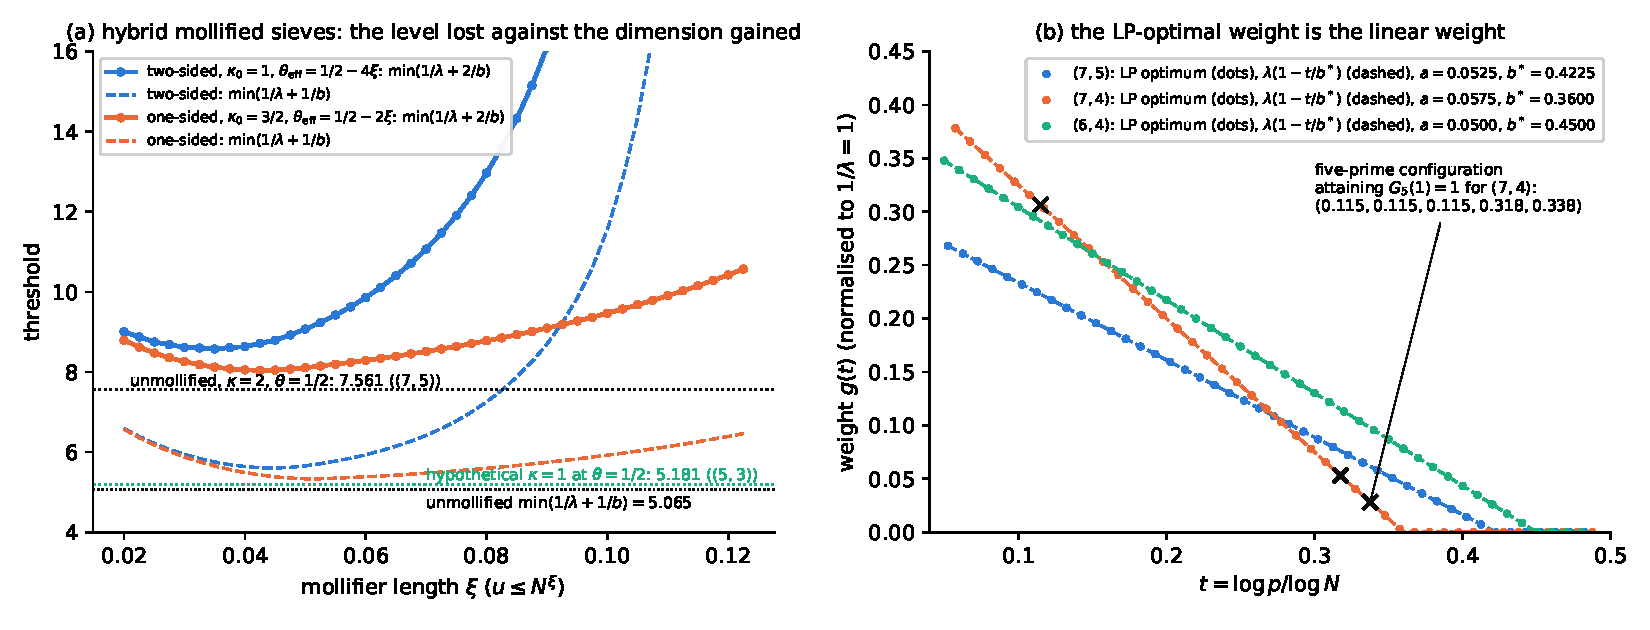
\includegraphics[width=\textwidth]{sieve_barriers.pdf}
\caption{(a) The best thresholds $\min(1/\lambda+2/b)$ (solid) and $\min(1/\lambda+1/b)$ (dashed) of the hybrid mollified sieves of Section~\ref{subsec:moll} against the mollifier length $\xi$, for the two-sided ($\kappa_0=1$, level $1/2-4\xi$) and the one-sided ($\kappa_0=3/2$, level $1/2-2\xi$) variants; dotted, the unmollified values $7.561$, $5.065$ at the level $1/2$ and the hypothetical dimension-one value $5.181$. (b) The LP-optimal weight $g^*(t)$ (dots) against the linear weight $\lambda(1-t/b^*)$ (dashed) for the pairs $(7,5)$, $(7,4)$, $(6,4)$ at the best $a$, normalised to $1/\lambda=1$; crosses, the five-prime configuration $(0.115,0.115,0.115,0.318,0.338)$ at which $G_5(1)=1$ binds $(7,4)$. Scripts \texttt{plot\_sieve\_barriers.py}, \texttt{mollified\_benchmark.py}, \texttt{optimal\_weights.py}; floating point.}
\label{fig:barriers}
\end{figure}

\subsection{Two further proposals}
\emph{The vector-sieve upper bound.} Since $p\mid n$ consumes the modulus $p$ on one side only, one might use, for $S(\cA_p,z)$, the vector sieve with levels $N^{\theta_A-t}$ and $N^{\theta-\theta_A}$ and the bound $\min_{\theta_A}F_1((\theta_A-t)/a)F_1((\theta-\theta_A)/a)$ in place of $F_2((\theta-t)/a)$. The two-dimensional sieve already allocates the whole level $N^{\theta-t}$ jointly, and for all $s\in[1,10]$
\[
F_2(s)\ \le\ \min_{s_A+s_B=s}F_1(s_A)F_1(s_B)
\]
(the ratio is at most $0.997$; for $s\le2$ it is $1/2$ exactly, since $F_2(s)=2(2e^\gamma)^2/s^2$ against $4e^{2\gamma}/(s_As_B)\ge16e^{2\gamma}/s^2$): nothing is gained.

\emph{Subtracting the five-prime integers.} The integers with $\Omega(n)=5$ that spoil $\max\Omega\le4$ have weight at most $1-\lambda G_5(1)$, which is small ($0.03$ at the best parameters), and one could try to bound their total contribution by an upper-bound sieve and subtract it. But an integer $n=p_1\cdots p_5$ with all $t_i\ge a$ and $\sum t_i\le1$ has $t_1+\cdots+t_4\ge1-\max t_i$, and the sieve that counts $\{n:\ p_1p_2p_3p_4\mid n\}$ has the level $N^{\theta-(t_1+\cdots+t_4)}$, which is below $N^{a}$ as soon as $t_1+\cdots+t_4>\theta-a$; the configurations that attain $G_5(1)$ have $t_1+\cdots+t_4\ge0.66>1/2$. So the dangerous integers lie outside the level, and the only handle on them is the weight itself.

\subsection{Pair weights}\label{subsec:pairs}
The programme above ranges over the separable weights $1-\lambda\sum_pg(t_p)$. The first alternative that stays inside the sieve is a weight with a term for each pair of prime factors,
\begin{equation}\label{eq:pairweight}
W(n)=1-\sum_{p\mid n(N-n)}g_1(t_p)-\sum_{\substack{p<q\\ pq\mid n(N-n)}}g_2(t_p,t_q),\qquad g_1,g_2\ge0
\end{equation}
($\lambda$ and $\mu$ absorbed into $g_1$ and $g_2$). The hope is combinatorial: a five-prime configuration has $\binom52=10$ pairs against the $\binom42=6$ of a four-prime one, where the single weights distinguish them only as $5$ against $4$, so a pair term could charge the configurations that bind $G_5(1)\ge1$ more selectively. The sieve accepts such weights, at the price that the pair $pq$ is sieved at the level $N^{\theta-t_p-t_q}$.

\begin{proposition}\label{prop:pairsieve}
Let $0<a<\theta$, $z=N^a$, $g_1\ge0$ bounded on $[a,1]$ with $g_1=0$ on $[b,1]$ for some $b<\theta$, $g_2\ge0$ bounded on $\{a\le u\le v:\ u+v\le\theta-a\}$ and zero elsewhere, both piecewise continuous, and $W$ as in \eqref{eq:pairweight}. Then
\begin{gather*}
\sum_{\substack{n\in\cA\\ (n(N-n),P(z))=1}}w(n)W(n)\ \ge\ X_NV(z)\Bigl(f_2\Bigl(\frac\theta a\Bigr)-R_1(g_1)-R_2(g_2)-o(1)\Bigr),\\
R_1(g_1)=2\int_a^bg_1(t)F_2\Bigl(\frac{\theta-t}a\Bigr)\frac{\dd t}t,\qquad R_2(g_2)=4\iint_{a\le u<v}g_2(u,v)F_2\Bigl(\frac{\theta-u-v}a\Bigr)\frac{\dd u\,\dd v}{uv}.
\end{gather*}
With
\[
G_k(S):=\inf\Bigl\{\sum_{i=1}^kg_1(t_i)+\sum_{1\le i<j\le k}g_2(t_i,t_j):\ t_i\ge a,\ t_1+\cdots+t_k\le S\Bigr\},
\]
non-decreasing in $k$ and non-increasing in $S$, the weight is $\le0$ on every $n$, square-free with all prime factors $\ge z$, that has $\Omega(n)>k'$ or $\Omega(N-n)>k'$ or $\Omega(n(N-n))>k$, as soon as
\begin{equation}\label{eq:Gcond2}
G_{k'+1}(1)\ \ge\ 1,\qquad G_{k_1}(1)+G_{k_2}(1)\ \ge\ 1\quad\text{for all }k_1+k_2=k+1,\ k_1,k_2\le k'.
\end{equation}
Hence, if $f_2(\theta/a)-R_1(g_1)-R_2(g_2)>0$ and \eqref{eq:Gcond2} holds at the level $\theta=1/2$, the conclusion of Part~II, Theorem~7.1, holds for the pair $(k,k')$.
\end{proposition}

\begin{proof}
Expanding the weight, the sum is $S(\cA,z)-\sum_pg_1(t_p)S(\cA_p,z)-\sum_{p<q}g_2(t_p,t_q)S(\cA_{pq},z)$ with $\cA_{pq}=\{n\in\cA:\ pq\mid n(N-n)\}$. For $(d,pq)=1$ one has $|\cA_{pq,d}|=X_N\,2h(p)\,2h(q)\prod_{\ell\mid d}2h(\ell)+R_{pqd}$ (Part~II, Section~7.2), so $\cA_{pq}$ is a sieve problem of dimension $2$ with the level $N^\theta/(pq)=N^{\theta-t_p-t_q}$, and the upper-bound sieve of Part~II, Section~7.1, gives $S(\cA_{pq},z)\le X_N\,2h(p)2h(q)\,V(z)\bigl(F_2((\theta-t_p-t_q)/a)+o(1)\bigr)$ plus a remainder; $g_2\ge0$ preserves the inequality, and $u+v\le\theta-a$ keeps the level at or above $z$, where $F_2$ is bounded. The remainders of all three sieves are sub-sums of $\sum_{m<N^\theta}\tau(m)^24^{\omega(m)}|R_m|$, which Part~I, Theorem~3.2 bounds by $N^{1-\e/3}$ (its condition (F1) admits every weight of size $N^{o(1)}$). The passage from $\sum_{p<q}2h(p)2h(q)\phi(t_p,t_q)$ to $\iint_{u<v}\phi(u,v)\,(2\,\dd u/u)(2\,\dd v/v)$ is that of Part~I, Section~4, in each variable, since $\sum_{p<z}2h(p)=2\log\log z+O(1)$; this gives $R_2$. For the positivity, an $n$ with $\Omega(n)\ge k'+1$ has $k'+1$ prime factors $t_i\ge a$ with $\sum t_i<1$; dropping the other primes and every pair that involves them lowers the penalty, since $g_1,g_2\ge0$, so the penalty is at least $G_{k'+1}(1)\ge1$. For $\Omega(n(N-n))\ge k+1$ with $\Omega(n)=k_1\le k'$ and $\Omega(N-n)\ge k_2=k+1-k_1$, drop in addition the pairs with one prime in $n$ and one in $N-n$: the penalty is at least $G_{k_1}(1)+G_{k_2}(1)\ge1$. The integers with $p^2\mid n(N-n)$ for some $p\ge z$ are negligible (Part~I, Lemma~4.1), and the conclusion follows as in Part~II, Section~7.2.
\end{proof}

The best margin for $(k,k')$ is now $f_2(\theta/a)-\min\{R_1(g_1)+R_2(g_2)\}$ over $g_1,g_2\ge0$ subject to \eqref{eq:Gcond2}: a linear programme in two unknown functions with one constraint per prime configuration, which for $g_2=0$ is the programme of Section~\ref{sec:optimal}. Its dual says when the pair term can help.

\begin{proposition}\label{prop:dual}
Fix nodes $t_l=a+l\delta$, $l\ge0$, with $a,1\in\delta\Z$, and consider $g_1$ continuous and piecewise linear with these nodes and $g_2$ constant on the cells $[t_l,t_{l+1})\times[t_m,t_{m+1})$, $l\le m$. The conditions \eqref{eq:Gcond2} restricted to the node configurations $t_i\in\{t_l\}$ are necessary, and they are sufficient when $g_2$ is non-increasing in each variable. The programme with the node conditions only is a finite linear programme in the node values $x_l$ of $g_1$ and the cell values $y_{lm}$ of $g_2$, with the costs $c_l=R_1(\text{hat function at }t_l)$, $c_{lm}=R_2(\mathbf 1_{\mathrm{cell}})$, and
\begin{multline*}
\min\Bigl\{\sum_lc_lx_l+\sum_{l\le m}c_{lm}y_{lm}\Bigr\}\\
=\max\Bigl\{\sum_\gamma r_\gamma\nu_\gamma:\ \nu\ge0,\ \ \sum_\gamma\nu_\gamma n_l(\gamma)\le c_l\ \ \forall l,\ \ \sum_\gamma\nu_\gamma n_{lm}(\gamma)\le c_{lm}\ \ \forall l\le m\Bigr\},
\end{multline*}
where $\gamma$ runs over the constraints \eqref{eq:Gcond2} at the node configurations (right-hand sides $r_\gamma=1$), $n_l(\gamma)$ is the number of primes of $\gamma$ at the node $t_l$ and $n_{lm}(\gamma)$ the number of its pairs, within one side, in the cell $(l,m)$. The separable programme ($y=0$) has the same dual without the pair constraints. Consequently the pair term lowers the minimal cost if and only if every optimal dual solution $\nu$ of the separable programme puts, on the pairs of primes in some cell $(l,m)$, more mass than $c_{lm}$; and if the two minima coincide, no $g_2\ge0$ constant on cells of size $\delta$, monotone or not, lowers the cost of the exact programme either.
\end{proposition}

\begin{proof}
On a product of cells the $g_2$-part of the penalty is constant and the $g_1$-part is linear in each $t_i$, so its infimum over the real configurations in that product with $\sum t_i\le1$ is attained at a vertex of (product of the closed cells) $\cap\{\sum t_i\le1\}$, and since $1-ka\in\delta\Z$ every coordinate of a vertex is a node. A coordinate at the right end of its cell is the node of the next cell, where $g_1$ takes its node value and $g_2$, if non-increasing, is not larger; so the infimum is at least the penalty of a node configuration. The programme with the node conditions is feasible and bounded below, so strong duality holds, and the dual of $\min\{c\cdot x:\ Ax\ge r,\ x\ge0\}$ is $\max\{r\cdot\nu:\ A^{\mathsf T}\nu\le c,\ \nu\ge0\}$, the columns of $A$ indexed by the pair cells being the counts $n_{lm}(\gamma)$. Removing the pair variables removes the corresponding dual constraints, and the two minima coincide if and only if some optimal dual solution of the smaller programme satisfies them. Finally the exact programme on these weights has more constraints than the node programme and contains the separable weights, so its minimum lies between the two.
\end{proof}

\emph{The solution.} The script \texttt{optimal\_weights\_2d.py} solves the node programme, with and without the monotonicity of $g_2$, at $\theta=1/2$ with $\delta=0.005$ (and $0.01$), $a\in\{0.05,0.055,0.06,0.065\}$, $g_1$ free on $[a,0.49)$ and $g_2$ free on the cells with $(\theta-u-v)/a\ge1$ (also $\ge1/2$). Since the pair term is not additive over the primes, the dynamic programme of Section~\ref{sec:optimal} no longer computes $G_k$; instead all node configurations of four and five primes with $\sum t_i\le1$ are enumerated ($1.1\cdot10^6$ and $5.3\cdot10^6$ at $\delta=0.005$) and the violated ones are added as cutting planes until none is left. The outcome for $(7,4)$ is the same at every $a$: the optimal weight has $g_2\equiv0$, and the margin is that of the separable programme, $-0.0599$, $-0.0355$, $-0.0303$, $-0.0472$ at $a=0.05,\dots,0.065$, with the linear $g_1$ of Section~\ref{subsec:lpresult}. The same holds with the pair support extended to $(\theta-u-v)/a\ge1/2$, without the monotonicity of $g_2$, at $\delta=0.01$, for $(6,4)$ ($-0.2266$ at $a=0.05$) and, at $\delta=0.01$, for $(7,5)$ ($+0.1173$ at $a=0.06$). Two further runs locate the reason. First, with every $F_2$ replaced by $1$ in the costs, so that the pair term carries no sieve penalty at all and the programme is the pure moment inequality for the Poisson model of the prime factors, the pair term is still not used: the separable optimum, now with the margin $+0.173$, is optimal among the pair weights as well. Second, multiplying the pair costs by $1-\varphi$, the pair cells enter the optimal weight only for $\varphi>0.4$; at $\varphi=0.6$ they move the margin from $-0.0303$ to $-0.0274$, and $(7,4)$ is reached ($+0.076$) only at $\varphi=0.8$, a pair term five times cheaper than the sieve gives (\texttt{results/optimal\_weights\_2d\_0.500\_0.005.txt}, \texttt{\dots\_0.01.txt}).

So the trade is not favourable, and not for the reason one would guess. The price $F_2((\theta-u-v)/a)$ is real ($F_2(4.5)=1.57$ for the pair $(0.115,0.115)$ at $a=0.06$, against $F_2(6.4)=1.06$ for the single prime $0.115$), but it does not decide: by Proposition~\ref{prop:dual}, some optimal dual measure $\nu$ of the separable programme, which lives on the five-prime configurations with $\sum t_i=1$ that saturate \eqref{eq:Gcond}, puts on the pairs of primes in every cell less mass than the cell costs, and it does so even when $F_2\equiv1$: the binding configurations are spread over the whole face $\sum t_i=1$ of the simplex, and a pair term, which charges a two-dimensional cell, catches too few of them for what it costs, so that it needs a discount of $40$ to $80$ per cent to enter at all. The leverage $10:6$ is correct, but what binds $(7,4)$ is not the number of primes, it is the budget $\sum t_i\le1$, and that budget the linear weight already exhausts ($G_k(1)=k-1/b$).

\subsection{Conclusion}
At the level $1/2$ with the Diamond--Halberstam--Richert functions, the linear programme finds no weight of the form $1-\lambda\sum_pg(t_p)$, $g\ge0$, that reaches $(7,4)$: on the grid (step $0.0025$, $a\in[0.045,0.075]$, support in $[a,0.49)$) the linear weight is optimal and its margin is $-0.030$; and no weight of the pair form \eqref{eq:pairweight} does better (Section~\ref{subsec:pairs}). This is numerical evidence, not a theorem: a proof for all admissible $g$ would be an LP dual certificate (a measure on prime configurations dominating the cost $2F_2((\theta-t)/a)/t$, as in Proposition~\ref{prop:dual}), which we have not constructed in closed form, and a continuous version would also have to allow the sieving limit $a$ to vary with $g$. What the evidence says is that the pair needs more level ($2/3$ gives $(6,4)$ with margin $0.196$) or a sieve input beyond $F_2,f_2$.

\emph{Scope of the linear programme, and the two exits inside the sieve.} The LP of Section~\ref{subsec:lpresult} ranges over the separable weights $1-\lambda\sum_pg(t_p)$, for which the weighted sieve reduces, through $\sum_pg(t_p)S(\cA_p,z)$, to upper bounds for the single-prime sequences $\cA_p$ at the level $N^{\theta-t_p}$ with the dimension-two function $F_2$. Two non-separable alternatives exist in principle. (a) \emph{Pair weights} $g_2(t_p,t_q)$ on $p,q\mid n(N-n)$: the sieve accepts them (Proposition~\ref{prop:pairsieve}), the programme extends to a two-dimensional grid, and its solution is the separable one, with $g_2\equiv0$, for the reason that Proposition~\ref{prop:dual} makes precise (Section~\ref{subsec:pairs}); within the inputs $F_2,f_2$ this exit is closed. (b) \emph{Chen's switching} \cite{ChenJR}: in Goldbach's problem the integers with three prime factors are bounded from above by sieving the switched sequence, and the dimension is thereby traded for a level of distribution on a sequence with a prime variable inside the modulus. Here (Section~\ref{subsec:dim}) the switched sequence is $\{pn'\}$ and its remainder is $\sum_{p\sim P}\bigl(T(dp,e;N)-M(dp,e;N)\bigr)$ for $de\le N^\theta$ and $P\ge N^b$, $b\approx0.4$: the sum over the sieve modulus $m=dp$ of the remainder $a_{G_{dp,e}}(N)$ with moduli up to $N^{\theta+b}>N^{1/2}$. This is the trilinear form \eqref{eq:trilinear} with the $m$-sum restricted to $m=dp$, i.e.\ the same object as in Sections~\ref{sec:dispersion}--\ref{sec:poisson}, with one additional structure, the bilinearity in $(d,p)$ that the prime variable provides (the arrangement of Linnik's problem, Remark~\ref{rem:disp}(iii)). So of the two exits from the $0.030$ that remain inside the sieve, the first leads to a larger linear programme with the same inputs, whose solution is the old one, and the second to the remainder problem of question (i): the switching principle does not circumvent the level of distribution, it requires it beyond $1/2$ on a bilinear sequence, and in the present problem that is the open question of Section~\ref{subsec:bilinear}, not an independent route.

\section{The level of distribution in short intervals}\label{sec:short}

Theorem~1.3 of Part~II gives the level $1-\e$ for all $N\equiv2\pmod4$ in $(X/2,X]$ outside an exceptional set of size $O(X^{1-\e/4})$; it says nothing about the $N$ in an interval of length $H<X^{1-\e/4}$, which could all be exceptional. The uniform bound gives the level $1/2$ for every single $N$. Here is what lies in between.

\subsection{The unconditional theorem}
\begin{theorem}\label{thm:short}
Let $0<\e<1/20$, $\e<\Delta\le1$, $X\ge X_0(\e)$, $H=X^\Delta$, $I=(X,X+H]$ and $D=X^{\Delta-3\e}$. Then
\[
\sum_{\substack{N\in I\\ N\equiv2\ (4)}}\ \sum_{\substack{de\le D,\ (d,e)=1\\ (de,2N)=1}}\mu^2(de)\,d_3(de)\,|R(d,e;N)|\ \ll_\e\ H\,X^{1-\e/2},
\]
and consequently all but $O_\e(HX^{-\e/4})$ of the integers $N\equiv2\pmod4$ in $I$ satisfy
\[
\sum_{\substack{de\le N^{\Delta-3\e}\\ (d,e)=1,\ (de,2N)=1}}\mu^2(de)\,d_3(de)\,|R(d,e;N)|\ \le\ N^{1-\e/5}:
\]
the level of distribution $\Delta-3\e$ for almost all $N$ in every interval of length $X^\Delta$.
\end{theorem}
\begin{proof}
We follow the proof of Theorem~1.3 (Part~II, Section~3.1) with $\eta=\e/10$. Insert the decomposition \eqref{eq:Rdecomp}. For the tuples with $t_1ss'>X^\e$ the trivial bound (Part~II, (5)) gives $|a_G(N')|\ll X^{2\eta}(X^{1-\e}/(de)+1)$ for each of the $H$ values of $N$, and summing over the $\le X^\eta$ tuples and over $de\le D$ with the weights $\le X^\eta$ these tuples contribute $\ll HX^{1+4\eta}\sum_{k\le D}d(k)(X^{1-\e}/k+1)\ll H(X^{2-\e+5\eta}+X^{1+5\eta}D)\ll HX^{1-\e/2}$, as $D\le X^{1-3\e}$. For the tuples with $t_1ss'\le X^\e$ the forms $G=G_{t_1m,m'}$ have level $L=4t_1ss'de\le4X^\e D\le X$, and for a fixed tuple and fixed $(d,e)$, Cauchy--Schwarz over the $\le H/t+1\le2H/t$ integers $N\in I$ with $t\mid N$ ($t\le X^\e\le H$) and Theorem~1.2 of Part~II on $[1,X+H]\subseteq[1,2X]$ give
\begin{multline*}
\sum_{\substack{N\in I\\ t\mid N}}\bigl(|a_G(N)|+|a_G(N/2)|\bigr)\le2\Bigl(\frac{2H}t\Bigr)^{1/2}\Bigl(\sum_{n\le2X}|a_G(n)|^2\Bigr)^{1/2}\\
\ll\Bigl(\frac Ht\Bigr)^{1/2}X\,(t_1ss'de)^{-1/2+\eta}\le H^{1/2}X^{1+\eta}\,t^{-1/2}(de)^{-1/2},
\end{multline*}
using $\sum_{n\le2X}|a_G(n)|^2\ll X^2\|G\|^2/L$ and $\|G\|^2\ll L^{\eta}$. Summing over $t\le X^\e$, the tuples and $de\le D$ as in Part~II,
\[
\ll H^{1/2}X^{1+4\eta+\e/2}\sum_{k\le D}d(k)k^{-1/2}\ll H^{1/2}X^{1+5\eta+\e/2}D^{1/2}=X^{\Delta/2+1+\e+\Delta/2-3\e/2}=HX^{1-\e/2}.
\]
The second assertion is Markov's inequality applied to $S(N)=\sum_{de\le D}\cdots$: the number of $N\in I$ with $S(N)>X^{1-\e/4}$ is $\ll HX^{1-\e/2}/X^{1-\e/4}=HX^{-\e/4}$, and for the others $N^{\Delta-3\e}\le D$ and $X^{1-\e/4}\le N^{1-\e/5}$.
\end{proof}

Theorem~\ref{thm:short} is trivial for $\Delta\le1/2$ (the level $1/2$ holds for every $N$) and gives, in every interval of length $X^\Delta$ with $\Delta>1/2$, the level $\Delta-3\e$ for almost all $N$: with the sieve of Part~II this is $(6,4)$ for almost all $N$ in intervals of length $X^{2/3+\e}$ (the parameters certified at the level $2/3$ in Part~II, Section~3) and $(5,4)$ in intervals of length $X^{19/20+\e}$. The unconditional threshold is therefore $H>X^{1/2}$: the proof uses the mean square of $a_G(n)$ over all $n\le2X$, which costs the factor $(X/H)^{1/2}$ against an average over the interval alone. For the arithmetic statement this range is superseded by the circle method, which produces $N=p+q$ with $p\equiv q\equiv1\pmod 4$ for almost all $N$ in intervals much shorter than $X^{1/2}$ (Perelli--Pintz \cite{PP} for the length $X^{7/36+\e}$ in the classical Goldbach setting, and shorter intervals in later work of Mikawa, Jia and Baker--Harman--Pintz; the extension to the residue class $1\pmod4$ has not been checked here); as for Theorem~1.3 of Part~II, the content is the level of distribution of the weighted sequence, not the arithmetic corollary.

\subsection{The missing input: a short-interval mean square}\label{subsec:missing}
The factor $(X/H)^{1/2}$ disappears if the mean square can be taken over the interval.

\begin{proposition}\label{prop:shortcond}
Let $0<\Delta<1$ and suppose that for every $L\le X$, every $G\in S_2(\Gamma_0(L))$ and every $H\in[X^\Delta,X]$,
\begin{equation}\label{eq:SDelta}
\sum_{X<n\le X+H}|a_G(n)|^2\ \ll_\eta\ X^{\eta}\,\frac{(H+L)\,X}{L}\,\|G\|^2 .
\end{equation}
Then Theorem~\ref{thm:short} holds with the level $\theta=(1+\Delta)/2-3\e$ in place of $\Delta-3\e$ (and $D=X^{\theta}$), for every $\Delta<1-3\e$.
\end{proposition}
\begin{proof}
In the Cauchy--Schwarz step, \eqref{eq:SDelta} replaces $X^2\|G\|^2/L$ by $X^{\eta}(H+L)X\|G\|^2/L$, so that the tuples with $t_1ss'\le X^\e$ contribute $\ll H^{1/2}X^{1/2+\e}\sum_{k\le D}d(k)(H+k)^{1/2}k^{-1/2}\ll H^{1/2}X^{1/2+2\e}(H^{1/2}D^{1/2}+D)$, since $(H+k)^{1/2}k^{-1/2}\le H^{1/2}k^{-1/2}+1$; the first term is $\ll HX^{1-\e/2}$ for $D\le X^{1-5\e}$ and the second for $D\le H^{1/2}X^{1/2-3\e}=X^{(1+\Delta)/2-3\e}$.
\end{proof}

So under \eqref{eq:SDelta} every $\Delta>0$ gives a level beyond $1/2$: $H=X^{1/3}$ would give $2/3$ and $(6,4)$, and the range $\Delta<7/36$, where the circle method no longer reaches, would give the level $\approx0.6$, still $(6,4)$. Everything therefore rests on \eqref{eq:SDelta}, which we now describe precisely.

\begin{enumerate}[label=\textup{(\alph*)},leftmargin=2.2em]
\item \emph{What it is.} For $\Delta=1$, \eqref{eq:SDelta} is Theorem~1.2 of Part~II (the covering argument), which is why Theorem~1.3 has the level $1-\e$. For $H<X$ the covering argument gives nothing: the weight $e^{-4\pi ny}$ of the Parseval integral is monotone in $n$, and a localisation of the coefficients to an interval of length $H<X$ needs an oscillating weight ($n^{it}$ with $|t|\le X/H$, i.e.\ the Eisenstein series $E(z,1+it)$ in the unfolding), whose convexity-type bounds $(1+|t|)^{1/2+\e}$ integrated over $|t|\le X/H$ cost far more than the factor $(X/H)^{1/2}$ they are meant to save.
\item \emph{Its spectral form.} With the Poincar\'e series $P_n$ of Part~II, Section~4 ($\langle f,P_n\rangle=a_f(n)/(4\pi n)$), $\sum_{n\in I}|a_G(n)|^2=\sum_{n\in I}(4\pi n)^2|\langle G,P_n\rangle|^2\le(4\pi(X+H))^2\|G\|^2\lambda_{\max}(M_I)$ with the Gram matrix $M_I=(\langle P_n,P_m\rangle)_{m,n\in I}$, and the bound is attained for $G$ the top eigenvector; so \eqref{eq:SDelta} is equivalent, up to $X^\eta$, to
\[
\lambda_{\max}(M_I)\ \ll\ X^{\eta}\,\frac{1+H/L}{X},\qquad\text{i.e.}\qquad\Bigl\|\sum_{n\in I}c_nP_n\Bigr\|^2\ll X^{\eta}\frac{1+H/L}{X}\sum_{n\in I}|c_n|^2 ,
\]
a large-sieve inequality for the Poincar\'e series of a short interval. It is sharp: $\tr M_I=\sum_{n\in I}\Delta_L(n,n)/(4\pi n)\asymp H/X$ and $\operatorname{rank}M_I\le\dim S_2(\Gamma_0(L))\asymp L$ give $\lambda_{\max}\gg H/(XL)$, and $P_N$ with $N<L$ (whose coefficient mass sits at $n=N$, Part~II, Section~4) gives $\lambda_{\max}\gg1/X$; the two together are the right-hand side.
\item \emph{Its Kloosterman form.} By Petersson's formula, $\langle P_n,P_m\rangle=\Delta_L(m,n)/(4\pi\sqrt{mn})$ with $\Delta_L(m,n)=\delta_{mn}-2\pi\sum_{c\equiv0\,(L)}c^{-1}S(m,n;c)J_1(4\pi\sqrt{mn}/c)$, so \eqref{eq:SDelta} asks for
\[
\sum_{c\equiv0\ (L)}\frac1c\sum_{m,n\in I}c_m\bar c_n\,S(m,n;c)\,J_1\Bigl(\frac{4\pi\sqrt{mn}}c\Bigr)\ \ll\ X^{\eta}\Bigl(1+\frac HL\Bigr)\|c\|^2 .
\]
The Weil bound gives $|\Delta_L(m,n)-\delta_{mn}|\ll X^{1/2+\eta}/L$ termwise, hence $\lambda_{\max}\ll(1+HX^{1/2+\eta}/L)/X$, which is useless (it does not even recover Theorem~1.2). The sum over $t\bmod c$ in $S(m,n;c)$ is a bilinear form in the exponential sums $\sum_{n\in I}c_ne(nt/c)$, and the additive large sieve bounds it by $(H+c)\|c\|^2$, which is the trivial $c\|c\|^2$ for $c\ge H$: for the moduli $c\equiv0\pmod L$ with $L\ge H$ there is no cancellation to be had inside a single Kloosterman sum, and the sum over the moduli $c\le X$ of the factors $c\cdot c^{-1}|J_1(4\pi X/c)|\asymp(c/X)^{1/2}$ (the trivial $c$ of the $t$-sum against the $1/c$ of Petersson's formula) then contributes $\asymp X/L$: this is the factor $(1+X/L)$ of the large sieve of Deshouillers--Iwaniec for coefficients supported on $n\le X$, i.e.\ Theorem~1.2 again. The gain from $H<X$ must come from cancellation in the sum over the moduli $c\equiv0\pmod L$ of the Bessel-weighted bilinear forms, with both arguments $m,n$ in the short interval. This is the obstacle of Section~\ref{subsec:deliver} in its symmetric form (two long arguments of length $H$ in place of one fixed argument $N$), which is the more favourable form, and it is exactly where the short-interval theory of Fourier coefficients (Jutila's method, the Voronoi summation in short intervals) would enter.
\item \emph{What the data say.} The quantity \eqref{eq:SDelta} is computable for the forms that matter. The script \texttt{short\_interval\_mean\_square.py} (\texttt{results/short\_interval\_mean\_square.txt}) takes the exact coefficients $a(n)=T-M$ of $G_{m,m'}$ for $n\le2^{21}$, the Rankin--Selberg mean $c(n)=16\pi^2\|G\|^2n/\vol(\Gamma_0(L)\backslash\HH)$ of $|a(n)|^2$, and computes
\[
\rho(X,H)=\frac{\sum_{X<n\le X+H}|a(n)|^2}{\sum_{X<n\le X+H}c(n)}
\]
for every window with $X\in[2^{19},2^{20}]$ (sliding, step $H/8$) and dyadic $H$ from $16$ to $2^{19}$, over all $n$ and over the admissible $n$ ($n\equiv2\pmod4$, $(n,mm')=1$), for seven pairs with $L$ from $20$ to $41612$. The mean of $\rho$ over the windows is $1.00$ for all $n$ (and $0.5$--$1.35$ for the admissible $n$, whose coefficients have a different mean), and the \emph{maximum} over the windows is
\begin{center}\small
\begin{tabular}{l|cccccc}
\toprule
$\max_X\rho(X,H)$, all $n$ & $H=16$ & $H=256$ & $H=2^{12}$ & $H=2^{14}$ & $H=2^{16}$ & $H=2^{19}$\\
\midrule
$(1,5)$, $L=20$ & $6.5$ & $1.67$ & $1.09$ & $1.04$ & $1.01$ & $1.00$\\
$(13,29)$, $L=1508$ & $5.7$ & $1.46$ & $1.08$ & $1.03$ & $1.01$ & $1.00$\\
$(1,10007)$, $L=40028$ & $4.3$ & $1.42$ & $1.11$ & $1.06$ & $1.05$ & $1.05$\\
$(101,103)$, $L=41612$ & $6.2$ & $1.50$ & $1.09$ & $1.07$ & $1.05$ & $1.02$\\
\bottomrule
\end{tabular}
\end{center}
with the same picture for the admissible $n$ (maxima $12$--$16$ at $H=16$, $1.3$--$1.5$ at $H=2^{12}$, $1.1$--$1.35$ at $H=2^{19}$). The decrease of the maximum with $H$ is the extreme-value statistics of $\asymp2^{19}\cdot8/H$ windows of $H$ terms of a heavy-tailed variable (kurtosis $3.5$--$3.8$, Part~II, Section~5.4), not a dependence on $L$: the columns are the same for $L=20$ and $L=4\cdot10^4$, and at $H=16$, where $H/L$ ranges from $0.8$ down to $0.0004$, the maxima are all between $4$ and $6.5$ (Figure~\ref{fig:short}(a)). So for the forms $G_{m,m'}$ the coefficient mass is spread at every scale down to $H\approx16$, and \eqref{eq:SDelta} holds with room to spare: the data support the stronger bound without the term $L$, which is needed only for the Poincar\'e series. This is the expected behaviour for a form that is ``generic'' with respect to the Poincar\'e basis, and it suggests proving \eqref{eq:SDelta} for $G_{m,m'}$ alone, through the arithmetic of $T-M$, rather than for all $G$: the left-hand side is the variance of the representation numbers $T(m,m';N)$ of the quaternary form over a short interval, $\sum_{N\in I}T(N)^2=\#\{(x,y)\in\Z^4\times\Z^4:\ Q(x)=Q(y)\in I\}$, a lattice-point problem for the indefinite form $Q\oplus(-Q)$ in eight variables. Section~\ref{subsec:lattice} shows that the required precision $HX/L$ is below what a circle-method treatment of this count can give, and that the lattice form reproduces the spectral problem rather than avoiding it.
\end{enumerate}

\subsection{The conjecture for the theta forms, and its consequence}
The data single out the statement that matters.

\begin{conjecture}[Short-interval mean square for the theta forms]\label{conj:short}
For coprime odd $m,m'$, $L=4mm'$, $G=G_{m,m'}$, $X\ge L$ and $X^{\eta}\le H\le X$,
\[
\sum_{X<n\le X+H}|a_G(n)|^2\ \ll_\eta\ X^{\eta}\,\frac{HX}{L}\,\|G\|^2 .
\]
\end{conjecture}

For $H=X$ this is Theorem~1.2 of Part~II; for $H=1$ it is Conjecture~4.1 of Part~II, the individual bound $|a_G(N)|\ll N^{1/2+\e}(mm')^{-1/2+\e}$; it says that the coefficient mass of $G_{m,m'}$ is spread at every scale, which is what Section~\ref{subsec:missing}(d) observes down to $H=16$. It is weaker than \eqref{eq:SDelta} in that it concerns one family of forms, and stronger in that it has no term $L$.

\begin{corollary}\label{cor:short}
Assume Conjecture~\ref{conj:short} for the forms $G_{t_1m,m'}$ of \eqref{eq:Rdecomp} with $t_1ss'\le X^\e$ and $H\ge X^{\e}$. Then Theorem~\ref{thm:short} holds with the level $1-3\e$, i.e.\ with $D=X^{1-3\e}$, for every $\Delta\in(\e,1]$: almost all $N\equiv2\pmod 4$ in every interval of length $X^\Delta$ have the level of distribution $1-\e$, and with it the pair $(5,4)$ of Part~II, Corollary~1.4 (and $(5,3)$ with the two-dimensional sieve of Part~II, Table~4, at the level $19/20$).
\end{corollary}
\begin{proof}
Without the term $L$ the Cauchy--Schwarz step gives, for every tuple and every $(d,e)$,
\[
\sum_{\substack{N\in I\\ t\mid N}}\bigl(|a_G(N)|+|a_G(N/2)|\bigr)\ll\Bigl(\frac Ht\Bigr)^{1/2}\Bigl(X^{\eta}\frac{HX}{L}\|G\|^2\Bigr)^{1/2}\ll HX^{1/2+2\eta}\,t^{-1/2}(de)^{-1/2},
\]
uniformly in $de\le D$ (the factor $k^{-1/2}$ is now present for every $k=de$, large or small), and the sum over $t$, the tuples and $k\le D$ is $\ll HX^{1/2+\e}\sum_{k\le D}d(k)k^{-1/2}\ll HX^{1/2+\e+\eta}D^{1/2}$, which is $\ll HX^{1-\e/2}$ for $D\le X^{1-3\e}$.
\end{proof}

\begin{remark}
The three statements of this section interpolate between the two results of Part~II: the level is $\Delta$ with the mean square over $[1,2X]$ (Theorem~\ref{thm:short}, unconditional, the covering argument), $(1+\Delta)/2$ with the mean square over the interval for all forms of level $L$ (Proposition~\ref{prop:shortcond}, the term $L$ accounting for the Poincar\'e series), and $1-\e$ with the mean square over the interval for the theta forms themselves (Corollary~\ref{cor:short}), which at $H=1$ is the individual conjecture of Part~II, Section~4, and at $H=X$ is Theorem~1.3 of Part~II. In the Poincar\'e-series language, \eqref{eq:SDelta} is a statement about the Gram matrix of the $P_n$, $n\in I$, and Conjecture~\ref{conj:short} about the position of the single vector $G_{m,m'}$ relative to that basis.
\end{remark}

\section{Spectral decomposition of the short-interval mean square: diagonal and off-diagonal}\label{sec:spectral}

Why do the Poincar\'e series need the term $L$ in \eqref{eq:SDelta} and the theta forms, numerically, not? The spectral expansion answers this exactly.

\subsection{The decomposition}
Let $\cB^*$ be an orthogonal basis of $S_2(\Gamma_0(L))$ consisting of eigenforms of all Hecke operators $T_p$, $p\nmid L$ (within each $S(f)$ an orthogonal basis of the span of the $f(\delta\,\cdot)$, for instance by Gram--Schmidt in the order of $\delta$). For $G\in S_2(\Gamma_0(L))$ write $G=\sum_{\varphi\in\cB^*}c_\varphi\varphi$, $c_\varphi=\langle G,\varphi\rangle/\|\varphi\|^2$, so that $a_G(n)=\sum_\varphi c_\varphi a_\varphi(n)$ and $\|G\|^2=\sum_\varphi|c_\varphi|^2\|\varphi\|^2$. For a weight $w_I\ge0$ supported on $(X,X+H]$,
\begin{gather}
\sum_nw_I(n)|a_G(n)|^2=\mathcal D_I(G)+\mathcal O_I(G),\qquad
\mathcal D_I(G)=\sum_{\varphi}|c_\varphi|^2\sum_nw_I(n)|a_\varphi(n)|^2,\label{eq:specdec}\\
\mathcal O_I(G)=\sum_{\varphi_1\ne\varphi_2}c_{\varphi_1}\bar c_{\varphi_2}\sum_nw_I(n)a_{\varphi_1}(n)\overline{a_{\varphi_2}(n)} .\notag
\end{gather}

The diagonal needs only an \emph{upper} bound for the short-interval mean square of each eigenform, not an asymptotic formula, and such an upper bound is available down to $H=X^\e$.

\begin{theorem}[The diagonal, eigenform by eigenform]\label{prop:diag}
Let $L\ge1$, $\e>0$, $X\ge2$, $X^{\e}\le H\le X$, and $0\le w_I\le1$ supported on $(X,X+H]$. Let $\varphi\in\cB^*$ and let $f$ be the newform, of level $M\mid L$, with $\varphi\in S(f)$. Then
\begin{equation}\label{eq:eigenms}
\sum_nw_I(n)|a_\varphi(n)|^2\ \ll_\e\ X^{\e}\,\frac{(H+L/M)\,X}{L}\,\|\varphi\|^2,
\end{equation}
and consequently, for every $G\in S_2(\Gamma_0(L))$, with $\pr_f$ the orthogonal projection onto $S(f)$,
\begin{equation}\label{eq:diagG}
\mathcal D_I(G)\ \ll_\e\ X^{\e}\,\frac XL\Bigl(H\|G\|^2+\sum_f\frac L{M_f}\|\pr_fG\|^2\Bigr)\ \le\ X^{\e}\,\frac{(H+L/M_G)\,X}{L}\,\|G\|^2,
\end{equation}
where $M_G$ is the smallest level of a newform $f$ with $\pr_fG\ne0$. In particular the newform components, and every $G$ in the range $H\ge L/M_G$, satisfy the bound $X^\e HX\|G\|^2/L$ of Conjecture~\ref{conj:short} without the term $L$.
\end{theorem}
\begin{proof}
The second statement follows from the first by Parseval, since the $\varphi\in\cB^*\cap S(f)$ are orthogonal:
\begin{multline*}
\mathcal D_I(G)=\sum_\varphi|c_\varphi|^2\sum_nw_I|a_\varphi(n)|^2\ll_\e X^\e\frac XL\sum_f\Bigl(H+\frac L{M_f}\Bigr)\sum_{\varphi\in\cB^*\cap S(f)}|c_\varphi|^2\|\varphi\|^2\\
=X^\e\frac XL\sum_f\Bigl(H+\frac L{M_f}\Bigr)\|\pr_fG\|^2 .
\end{multline*}
For the first, normalise $f$ by $a_f(1)=1$. Three inputs.

(a) \emph{Deligne's bound} \cite{Deligne}: $|a_f(n)|\le d(n)n^{1/2}$ for all $n$ (at $p\mid M$ one has $|a_f(p^\ell)|\le1$, so the bound holds for all $n$, not only for $(n,M)=1$).

(b) \emph{Shiu's theorem} \cite[Theorem~1]{Shiu}: for a non-negative multiplicative function with $g(p^\ell)\le A^\ell$ and $g(n)\ll_\delta n^\delta$, and for $Y^{\e}\le H'\le Y$, $\sum_{Y<m\le Y+H'}g(m)\ll_{\e}(H'/\log Y)\exp\bigl(\sum_{p\le Y}g(p)/p\bigr)$. With $g=d^2$ ($d(p^\ell)^2=(\ell+1)^2\le4^\ell$, $\sum_{p\le Y}4/p=4\log\log Y+O(1)$) this gives $\sum_{Y<m\le Y+H'}d(m)^2\ll_\e H'(\log Y)^3$. The sum $\sum_nw_I(n)|a_f(n/\delta)|^2$ runs over the $m=n/\delta$ in $(X/\delta,(X+H)/\delta]$, an interval of length $H/\delta$, which is at least $(X/\delta)^{\e/2}$ when $\delta\le H^{1/2}$; then (a) and Shiu's theorem give $\ll_\e(H/\delta)(X/\delta)(\log X)^3$. When $\delta>H^{1/2}$ the theorem does not apply, and we use the trivial bound: the interval contains at most $H/\delta+1$ integers $m$, each with $d(m)^2m\ll_\e X^{\e}X/\delta$. In all cases
\[
\sum_nw_I(n)|a_f(n/\delta)|^2\ \ll_\e\ X^{\e}\Bigl(\frac H\delta+1\Bigr)\frac X\delta=X^{\e}\,\frac{(H+\delta)X}{\delta^2}\qquad(\delta\ge1);
\]
the term $\delta$ is real, since an interval shorter than $\delta$ contains at most one multiple of $\delta$, whose coefficient is of size $(X/\delta)^{1/2}$ and not smaller.

(c) \emph{The norms.} By the Rankin--Selberg unfolding, the residue at $s=2$ of $\sum_n|a_f(n)|^2n^{-s}$ is $(4\pi)^2\|f\|^2_{\Gamma_0(M)}/\vol(\Gamma_0(M)\backslash\HH)$ and equals $L(1,\mathrm{sym}^2f)$ times $\zeta(2)^{-1}$ and local factors at $p\mid M$ bounded above and below by absolute constants; with $\vol(\Gamma_0(M)\backslash\HH)=\frac\pi3M\prod_{p\mid M}(1+1/p)$ and $(\log M)^{-1}\ll L(1,\mathrm{sym}^2f)\ll(\log M)^3$ (Hoffstein--Lockhart \cite{HL} for the lower bound) this is $\|f\|^2_{\Gamma_0(M)}=M^{1+o(1)}$. Since $\|f\|^2_{\Gamma_0(L)}=[\Gamma_0(M):\Gamma_0(L)]\,\|f\|^2_{\Gamma_0(M)}$ and $\|f(\delta\,\cdot)\|^2_{\Gamma_0(L)}=\delta^{-2}\|f\|^2_{\Gamma_0(L)}$ for $\delta\mid L/M$ (weight $2$), the unit vectors $u_\delta=f(\delta\,\cdot)/\|f(\delta\,\cdot)\|$ satisfy, by (b),
\[
\sum_nw_I(n)|a_{u_\delta}(n)|^2\ \ll_\e\ X^{\e}\,\frac{(H+\delta)X/\delta^2}{\delta^{-2}L^{1+o(1)}}\ =\ X^{\e+o(1)}\frac{(H+\delta)X}{L}\qquad(\delta\mid L/M).
\]
It remains to pass from the $u_\delta$ to the orthogonal basis $\cB^*\cap S(f)$. Let $\Gamma=(\langle u_{\delta_1},u_{\delta_2}\rangle)_{\delta_1,\delta_2\mid L/M}$ be the Gram matrix. By the inner-product formulae of \cite[Section~2]{ILS}, $\langle u_{\delta_1},u_{\delta_2}\rangle$ depends only on the local data of $\delta_2/\delta_1$ and $(\delta_1,\delta_2)$ at each prime, so that $\Gamma=\bigotimes_{p\mid L/M}\Gamma_p$ with $\Gamma_p$ of size $v_p(L/M)+1$; for $p\nmid M$ the off-diagonal entry at distance one is $\rho_f(p)=\lambda_f(p)/(p^{1/2}(1+1/p))$, so $|\rho_f(p)|\le2\sqrt p/(p+1)<1$, for $p\mid M$ it is $\lambda_f(p)$ with $|\lambda_f(p)|\le p^{-1/2}$, and the entries at distance $j\ge2$ are $\ll_j p^{-j/2}$. Hence $\lambda_{\min}(\Gamma_p)\ge1-Cp^{-1/2}$ for $p\ge p_0$ (Gershgorin), and $\lambda_{\min}(\Gamma_p)\ge c_0>0$ for $p<p_0$ (the finitely many local matrices are positive definite, being Gram matrices of linearly independent functions, and depend continuously on $\lambda_f(p)\in[-2,2]$), so that
\[
\lambda_{\min}(\Gamma)=\prod_{p\mid L/M}\lambda_{\min}(\Gamma_p)\ \ge\ \exp\Bigl(-C'\sum_{p\mid L/M}p^{-1/2}\Bigr)\ \ge\ L^{-o(1)},
\]
because $\sum_{p\mid n}p^{-1/2}\ll\sqrt{\omega(n)\log\omega(n)}=o(\log n)$. Now any $\varphi\in S(f)$ is $\varphi=\sum_\delta y_\delta u_\delta$ with $\|\varphi\|^2=y^{\mathrm t}\Gamma\bar y\ge\lambda_{\min}(\Gamma)|y|^2$, and by Cauchy--Schwarz
\begin{multline*}
\sum_nw_I(n)|a_\varphi(n)|^2\le\Bigl(\sum_\delta|y_\delta|\bigl(\sum_nw_I|a_{u_\delta}(n)|^2\bigr)^{1/2}\Bigr)^2\\
\le d(L/M)\,|y|^2\,X^{\e+o(1)}\max_{\delta\mid L/M}\frac{(H+\delta)X}{L}\le X^{\e+o(1)}\frac{(H+L/M)X}{L}\,\frac{\|\varphi\|^2}{\lambda_{\min}(\Gamma)},
\end{multline*}
which is \eqref{eq:eigenms}.
\end{proof}

The term $L/M$ in \eqref{eq:eigenms} is the price of the oldforms: $f(\delta\,\cdot)$ is supported on $\delta\Z$, and a window shorter than $\delta$ sees at most one of its coefficients, of size $(X/\delta)^{1/2}$, against a norm $\delta^{-1}\|f\|_L$. For the theta forms it is harmless, because their oldform components of small level have small norm, by the Rankin--Selberg formula of Part~II.

\begin{proposition}[The diagonal of the theta forms carries no term $L$]\label{prop:diagtheta}
Let $m,m'$ be coprime odd square-free integers, $n=mm'$, $L=4n$, $G=G_{m,m'}$, and $X^{\e}\le H\le X$. Then
\[
\mathcal D_I(G_{m,m'})\ \ll_\e\ X^{\e}\,\frac{HX}{L}\,\|G_{m,m'}\|^2 .
\]
\end{proposition}
\begin{proof}
By \eqref{eq:diagG} and $\|G\|^2\ge\frac1\pi(\log n)^2$ (Part~II, Theorem~1.5) it suffices to show that
\[
\sum_f\frac L{M_f}\|\pr_fG\|^2\ \ll\ n^{o(1)} .
\]
Let $f$ be a newform of level $M=2^eM_1$, $M_1\mid n$. Part~II, Theorem~6.7(ii) gives $\langle\Theta_{1,n},f(d\,\cdot)\rangle=\kappa_f/d$ for $d\mid L/M$, where $\kappa_f$ is $0$ or of modulus $\frac4{\pi^2}2^{r}|L(1,f)L(1,f\otimes\chi)|$, $r=\omega(n/M_1)$, and (iii) that the same holds for $\Theta_{m,m'}$ up to a sign common to all $d$. Since $E\perp S(f)$, $\pr_fG=\pr_f\Theta$, and in terms of the Gram matrix $\Gamma$ of the unit vectors $u_d$ of the proof of Theorem~\ref{prop:diag} and $\|f(d\,\cdot)\|_L=d^{-1}\|f\|_L$ one finds
\[
\|\pr_fG_{m,m'}\|^2=\frac{\kappa_f^2\ \mathbf 1^{\mathsf T}\Gamma^{-1}\mathbf 1}{\|f\|_L^2},\qquad 1\le\mathbf 1^{\mathsf T}\Gamma^{-1}\mathbf 1\le\frac{d(L/M)}{\lambda_{\min}(\Gamma)}\le L^{o(1)},
\]
($\mathbf 1$ the all-ones vector; the lower bound is $|\mathbf 1|^2/\lambda_{\max}(\Gamma)$ with $\lambda_{\max}\le\tr\Gamma=d(L/M)$). With $\|f\|_L^2\ge(L/M)\|f\|_M^2=(L/M)M^{1+o(1)}$ this gives
\[
\frac LM\|\pr_fG_{m,m'}\|^2\ \le\ n^{o(1)}\,\frac{L(1,f)^2L(1,f\otimes\chi)^2}{M_1}.
\]
On the other hand, the same formula for $n'=M_1$, which is odd and square-free and for which $|\kappa_f|=\frac4{\pi^2}|L(1,f)L(1,f\otimes\chi)|$ exactly, together with $\|f\|^2_{4M_1}\le6\|f\|_M^2=M_1^{1+o(1)}$, gives
\[
\|\pr_fG_{1,M_1}\|^2\ \ge\ M_1^{-1-o(1)}\,L(1,f)^2L(1,f\otimes\chi)^2 .
\]
Hence, the $S(f)$ being orthogonal,
\[
\sum_f\frac L{M_f}\|\pr_fG_{m,m'}\|^2\ \le\ n^{o(1)}\sum_{M_1\mid n}\ \sum_{f:\ M_1(f)=M_1}\|\pr_fG_{1,M_1}\|^2\ \le\ n^{o(1)}\sum_{M_1\mid n}\|G_{1,M_1}\|^2\ \ll\ n^{o(1)},
\]
by $\|G_{1,M_1}\|^2\ll M_1^{\e}$ (Part~I, Theorem~1.2; Part~II, Theorem~1.1(i)) and $d(n)=n^{o(1)}$.
\end{proof}

\begin{corollary}\label{cor:equiv}
For $G=G_{m,m'}$, $L=4mm'$, and $X^\eta\le H\le X$, Conjecture~\ref{conj:short} is equivalent to the off-diagonal bound
\begin{equation}\label{eq:offbound}
|\mathcal O_I(G_{m,m'})|\ \ll_\eta\ X^{\eta}\,\frac{HX}{L}\,\|G_{m,m'}\|^2 .
\end{equation}
\end{corollary}
\begin{proof}
$\sum_nw_I|a_G|^2=\mathcal D_I+\mathcal O_I$ and Proposition~\ref{prop:diagtheta} bounds $\mathcal D_I$ by the right-hand side of \eqref{eq:offbound} in both directions of the equivalence.
\end{proof}

\begin{remark}\label{rem:trivial}
(i) Cauchy--Schwarz over the basis gives the trivial bound:
\[
\sum_nw_I|a_G(n)|^2\le\Bigl(\sum_\varphi|c_\varphi|\bigl(\sum_nw_I|a_\varphi|^2\bigr)^{1/2}\Bigr)^2\le|\cB^*|\,\mathcal D_I(G),
\]
and $|\cB^*|=\dim S_2(\Gamma_0(L))\ll L$: so, by Proposition~\ref{prop:diagtheta}, $\sum_{X<n\le X+H}|a_G(n)|^2\ll X^\e HX\|G\|^2$ for the theta forms and every $H\ge1$ (a window shorter than $X^\e$ is contained in one of length $X^\e$), which is Conjecture~\ref{conj:short} without the factor $1/L$. At $H=1$ this reads $|a_G(N)|^2\ll N^{1+\e}\|G\|^2$: the uniform bound of Part~I (Part~II, Theorem~1.1(ii)), up to the norm, is the spectral trivial bound. Conjecture~\ref{conj:short} is therefore exactly the saving of the factor $L$ on the off-diagonal, i.e.\ square-root cancellation over the $\asymp L^2$ ordered pairs $(\varphi_1,\varphi_2)$ in \eqref{eq:offbound}, uniformly in the windows.

(ii) The classical short-interval \emph{asymptotic} $\sum_{X<n\le X+H}|a_\varphi(n)|^2\sim c_\varphi HX$ is known only for $H\ge X^{3/5+\e}$ (the Rankin--Selberg error term $O(X^{8/5})$), and the Lindel\"of hypothesis for $L(s,\varphi\times\bar\varphi)$ would give it for $H\ge X^{1/2+\e}$; neither is needed. The term $L$ in \eqref{eq:SDelta} cannot come from the diagonal; it is an off-diagonal phenomenon, and Table~\ref{tab:spectral} measures \eqref{eq:offbound} directly: the ratio $S_{\mathrm{off}}/S_{\mathrm{diag}}$ has mean $\le0.006$ and root mean square decreasing like $H^{-1/2}$, i.e.\ the off-diagonal behaves like a sum of $H$ uncorrelated terms of the size of a single diagonal term, which is the content of \eqref{eq:offbound} for the forms tested.
\end{remark}

\subsection{The mechanism: coherence against decorrelation}
\begin{proposition}\label{prop:mechanism}
\begin{enumerate}[label=\textup{(\roman*)},leftmargin=2.2em]
\item For the Poincar\'e series $G=P_N$, $c_\varphi=\overline{a_\varphi(N)}/(4\pi N\|\varphi\|^2)$, and at $n=N$ every off-diagonal term is non-negative:
\[
c_{\varphi_1}\bar c_{\varphi_2}a_{\varphi_1}(N)\overline{a_{\varphi_2}(N)}=\frac{|a_{\varphi_1}(N)|^2|a_{\varphi_2}(N)|^2}{(4\pi N)^2\|\varphi_1\|^2\|\varphi_2\|^2}\ \ge0 .
\]
Hence $|a_{P_N}(N)|^2=\bigl(\sum_\varphi|a_\varphi(N)|^2/(4\pi N\|\varphi\|^2)\bigr)^2$, whose off-diagonal part exceeds its diagonal part by the factor $\asymp\#\{\varphi:\ |a_\varphi(N)|^2/\|\varphi\|^2\asymp\text{typical}\}\asymp\dim S_2(\Gamma_0(L))\asymp L$ when the normalised coefficients at $N$ are of comparable size; this coherent alignment at the single index $n=N$ is the source of the term $L$ in \eqref{eq:SDelta}, and of the lower bound $\lambda_{\max}(M_I)\gg1/X$.
\item For $G=G_{m,m'}$ with $mm'$ square-free, the coefficients $c_\varphi$ are, by Theorem~6.7 of Part~II and Proposition~6.19 there, explicit combinations of the central values $L(1,f)L(1,f\otimes\chi)$ of the newforms $f$ underlying $\varphi$, with signs $\chi(\cdot)\eta_\cdot(f)$ and Gram-matrix factors: they do not depend on $X$, $H$ or $N$. The off-diagonal part is therefore
\[
\mathcal O_I(G_{m,m'})=\sum_{\varphi_1\ne\varphi_2}c_{\varphi_1}\bar c_{\varphi_2}\,\sum_nw_I(n)a_{\varphi_1}(n)\overline{a_{\varphi_2}(n)},
\]
a fixed quadratic form in the short-interval correlations of distinct eigenforms, which have mean zero over $X$ (for $\varphi_1\ne\varphi_2$ with distinct Hecke eigenvalues the Rankin--Selberg series $\sum_na_{\varphi_1}(n)\overline{a_{\varphi_2}(n)}n^{-s}$ has no pole at $s=2$, so $\sum_{n\le X}a_{\varphi_1}(n)\overline{a_{\varphi_2}(n)}=o(X^2)$). By Corollary~\ref{cor:equiv}, Conjecture~\ref{conj:short} is the bound \eqref{eq:offbound} for this quadratic form, uniformly in the windows: the family of eigenforms, weighted by the central values, is spectrally decorrelated on short intervals.
\end{enumerate}
\end{proposition}
\begin{proof}
(i) is the definition of $P_N$, $\langle f,P_N\rangle=a_f(N)/(4\pi N)$, applied to $f=\varphi$ and expanded; the expression for $a_{P_N}(N)$ is $\sum_\varphi c_\varphi a_\varphi(N)$. (ii) restates \eqref{eq:specdec} with the coefficients of Part~II; the mean-zero statement is the Rankin--Selberg method for two distinct eigenforms, and the last sentence is Corollary~\ref{cor:equiv}.
\end{proof}

So the difference between the two cases is not in the eigenforms but in the coefficients: the Poincar\'e series is, by construction, the vector that aligns all spectral phases at one index, and the theta forms have phases fixed by arithmetic (central values), with no index singled out. Conjecture~\ref{conj:short} says that this arithmetic family does not align by accident in any window.

\subsection{Numerical verification}
The script \texttt{short\_interval\_spectral.py} isolates the $T_3$-eigencomponents $v_i$ of $G_{1,q}$ by Prony's method on $(T_3^kG)(1)$, as in \texttt{newform\_support.py} of Part~II, for the levels $4q$ with at most five components (for $q=13,17,29,37$ these contain one to three newforms of level $4q$ and old components, for $q=19,23,31,43$ old components only); distinct Hecke eigenvalues make the $v_i$ orthogonal, so $G=\sum_iv_i$ is a decomposition of the type \eqref{eq:specdec} (coarser than $\cB^*$ when a $T_3$-eigenspace contains several Hecke components, which only moves part of the off-diagonal into the diagonal). For sliding windows $(X,X+H]$ with $X\in[2^{14},2^{15}]$ it computes
\[
S_{\mathrm{total}}=\sum_{n\in I}|a_G(n)|^2,\qquad S_{\mathrm{diag}}=\sum_i\sum_{n\in I}|a_{v_i}(n)|^2,\qquad S_{\mathrm{off}}=S_{\mathrm{total}}-S_{\mathrm{diag}},
\]
and, for comparison, the aligned model $P(n)=\sum_i\operatorname{sgn}(a_{v_i}(N_0))\,a_{v_i}(n)$ with $N_0$ the centre of the window, which has the same diagonal and is coherent at $n=N_0$. Table~\ref{tab:spectral} gives the mean and the root mean square of $S_{\mathrm{off}}/S_{\mathrm{diag}}$ over the windows (\texttt{results/short\_interval\_spectral.txt}); Figure~\ref{fig:short}(b) shows the two trajectories for $G_{1,29}$.

\begin{table}[htbp]
\centering\footnotesize
\setlength{\tabcolsep}{4pt}
\begin{tabular}{ccc|cccc|c}
\toprule
$q$ & level & comp. & $H=16$ & $H=256$ & $H=4096$ & $H=16384$ & model, max at $H=16$\\
\midrule
$13$ & $52$ & $2$ & $-0.001\ (0.158)$ & $-0.000\ (0.040)$ & $+0.001\ (0.006)$ & $+0.001\ (0.003)$ & $0.84$\\
$17$ & $68$ & $3$ & $+0.001\ (0.203)$ & $-0.000\ (0.052)$ & $-0.003\ (0.012)$ & $+0.000\ (0.003)$ & $0.83$\\
$29$ & $116$ & $4$ & $+0.004\ (0.274)$ & $+0.005\ (0.058)$ & $+0.003\ (0.009)$ & $-0.000\ (0.003)$ & $1.18$\\
$37$ & $148$ & $4$ & $-0.005\ (0.266)$ & $-0.003\ (0.067)$ & $-0.004\ (0.015)$ & $-0.001\ (0.005)$ & $1.18$\\
$19$ & $76$ & $2$ & $+0.000\ (0.246)$ & $+0.000\ (0.062)$ & $+0.003\ (0.018)$ & $+0.002\ (0.003)$ & $0.80$\\
$23$ & $92$ & $3$ & $+0.002\ (0.249)$ & $+0.000\ (0.067)$ & $+0.000\ (0.009)$ & $-0.001\ (0.002)$ & $1.16$\\
$31$ & $124$ & $4$ & $+0.001\ (0.257)$ & $+0.000\ (0.066)$ & $+0.001\ (0.017)$ & $+0.000\ (0.003)$ & $1.15$\\
$43$ & $172$ & $4$ & $+0.003\ (0.278)$ & $+0.002\ (0.059)$ & $+0.003\ (0.013)$ & $-0.003\ (0.007)$ & $1.37$\\
\bottomrule
\end{tabular}
\caption{The spectral off-diagonal of the short-interval mean square of $G_{1,q}$ relative to the diagonal, over sliding windows of length $H$ with $X\in[2^{14},2^{15}]$: mean (root mean square) of $S_{\mathrm{off}}/S_{\mathrm{diag}}$ for $G_{1,q}$, and the maximum of the same ratio for the aligned model $P$ at $H=16$. Floating point.}
\label{tab:spectral}
\end{table}

At every level and every window length the off-diagonal averages to zero (the means are $\le0.006$ in absolute value, against root mean squares of $0.16$--$0.28$ at $H=16$ and $0.003$--$0.007$ at $H=16384$), its root mean square decreases like $H^{-1/2}$ as for a sum of $H$ uncorrelated terms, and its extreme values stay below the diagonal ($|S_{\mathrm{off}}|/S_{\mathrm{diag}}\le1.4$ at $H=16$, $\le0.21$ at $H=256$, $\le0.1$ at $H=1024$): the eigenform correlations $\sum_{n\in I}a_{v_i}(n)a_{v_j}(n)$ behave, with the window-independent coefficients of $G_{1,q}$, like independent signs, exactly as Proposition~\ref{prop:mechanism}(ii) describes. The aligned model, which flips the signs of the components so that they add up at the centre of the window, does not change this picture beyond the shortest windows (its means are again $\le0.06$, its maxima at $H=16$ are $0.8$--$1.4$): aligning the phases at a single index affects a window sum only through that index, and to inflate a short-interval mean square by a factor of the order of the dimension one needs what the Poincar\'e series has and the theta forms lack, a coefficient vector that concentrates the whole norm on one index. The whole-range ratio $S_{\mathrm{off}}/S_{\mathrm{diag}}$ over $n\le2^{16}$ is between $-0.0025$ and $+0.0021$ at all eight levels, which is the orthogonality of the components.

\begin{figure}[htbp]
\centering
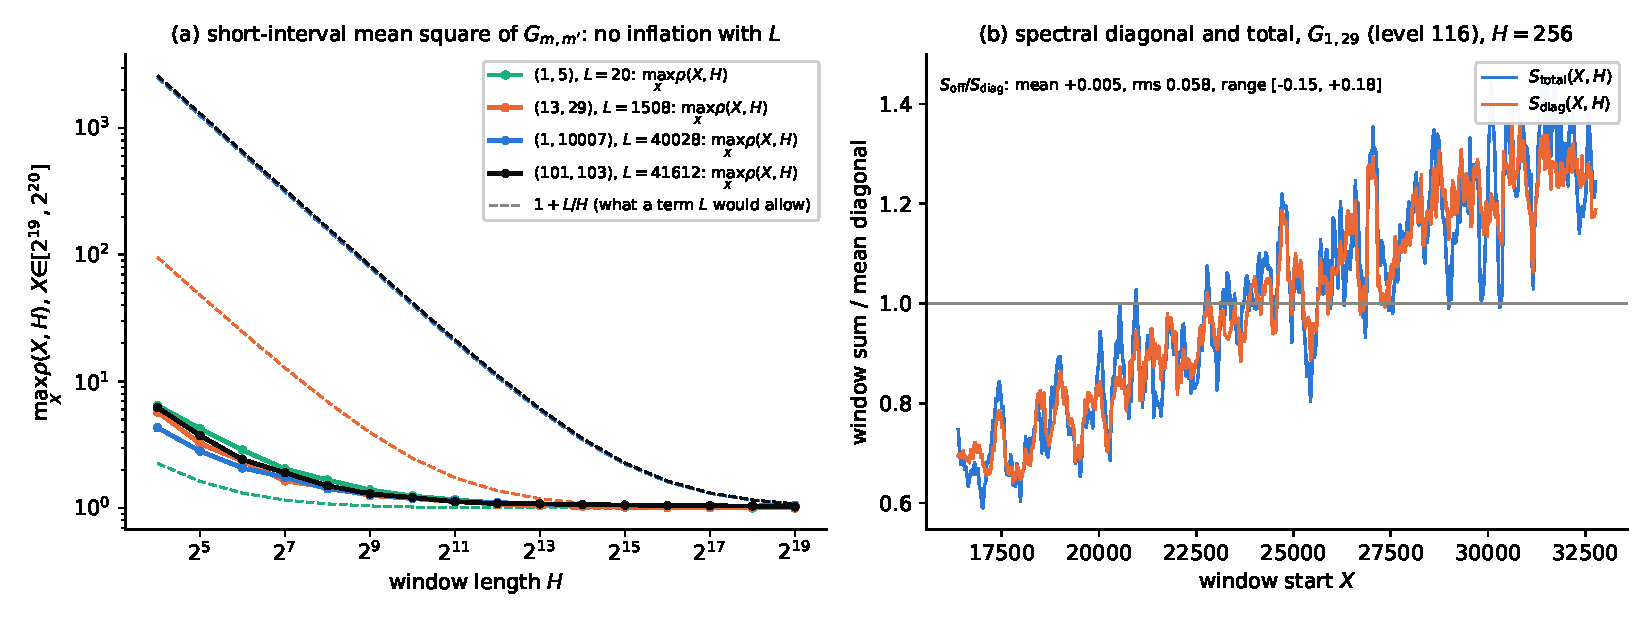
\includegraphics[width=\textwidth]{short_interval.pdf}
\caption{(a) The maximal window ratio $\max_X\rho(X,H)$ of the short-interval mean square of $G_{m,m'}$ against $H$ (log--log) for $L=20$, $1508$, $40028$, $41612$; dashed, the inflation $1+L/H$ that a term $L$ in \eqref{eq:SDelta} would allow. (b) The total $S_{\mathrm{total}}$ and the spectral diagonal $S_{\mathrm{diag}}$ of the short-interval mean square of $G_{1,29}$ (level $116$, four components) along sliding windows of length $256$, normalised by the mean diagonal. Scripts \texttt{plot\_short\_interval.py}, \texttt{short\_interval\_mean\_square.py}, \texttt{short\_interval\_spectral.py}; floating point.}
\label{fig:short}
\end{figure}

\subsection{The lattice-point form of the variance, and the precision it requires}\label{subsec:lattice}
Section~\ref{subsec:missing}(d) raised the question whether Conjecture~\ref{conj:short} for $G=G_{m,m'}$ could be proved through the lattice-point interpretation of $T-M$, bypassing the spectral expansion. It cannot, in the following precise sense. Write $Q=Q_{m,m'}=m(x_1^2+x_2^2)+m'(x_3^2+x_4^2)$, $T(N)=T(m,m';N)=\#\{x\in\Z^4:\ Q(x)=N\}$, $M(N)=M(m,m';N)$ the Siegel main term, $a_G=T-M$, $I=(X,X+H]$, and
\[
\mathcal T_I=\#\{(x,y)\in\Z^4\times\Z^4:\ Q(x)=Q(y)\in I\},\qquad V_I=\sum_{N\in I}a_G(N)^2 .
\]

Here $M(N)=\pi^2N\,\mathfrak S(N)/(mm')$ with the singular series
\[
\mathfrak S(N)=\sum_{q\ge1}q^{-4}\sum_{a\bmod q}^*S_q(a)\,e(-aN/q),\qquad S_q(a)=\sum_{x\bmod q}e\bigl(aQ(x)/q\bigr),
\]
so that $\mathfrak S(N)\ll N^{o(1)}$ and $\mathfrak S(N)\gg1$ for $N$ in the admissible classes, and $\sum_{N\in I}M(N)^2=HX^2L^{-2}X^{o(1)}$ for $H\ge X^\e$. The target is $V_I\ll X^\eta HX\|G\|^2/L$ (Conjecture~\ref{conj:short}), a relative precision $L/X$ against the main term, and the trivial bound is $V_I\ll HX^{1+\e}\|G\|^2$ (Remark~\ref{rem:trivial}(i)).

\begin{proposition}\label{prop:lattice}
\begin{enumerate}[label=\textup{(\roman*)},leftmargin=2.2em]
\item $V_I=\mathcal T_I-\sum_{N\in I}M(N)^2-2\sum_{N\in I}M(N)a_G(N)$, exactly.
\item $\bigl|\sum_{N\in I}M(N)a_G(N)\bigr|\le\bigl(\sum_{N\in I}M(N)^2\bigr)^{1/2}V_I^{1/2}$, hence $V_I\le2\,\bigl|\mathcal T_I-\sum_{N\in I}M(N)^2\bigr|+4\sum_{N\in I}M(N)^2$: with the cross term estimated by Cauchy--Schwarz, (i) gives nothing better than $V_I\ll HX^{2+o(1)}/L^2$, which is weaker than the trivial bound for $L\le X^{1/2}$.
\item To reach the bound of Conjecture~\ref{conj:short} from (i) one needs, besides $\mathcal T_I-\sum_{N\in I}M(N)^2\ll X^\eta HX\|G\|^2/L$, the bound
\begin{equation}\label{eq:cross}
\sum_{N\in I}M(N)a_G(N)=\frac{\pi^2}{mm'}\sum_{q\ge1}q^{-4}\sum_{a\bmod q}^*S_q(a)\sum_{N\in I}N\,a_G(N)\,e(-aN/q)\ \ll\ X^\eta\frac{HX}{L}\|G\|^2,
\end{equation}
a family of additively twisted first moments of $a_G$ over the window, each of which has the trivial bound $X\sum_{N\in I}|a_G(N)|\le XH^{1/2}V_I^{1/2}$; if Conjecture~\ref{conj:short} holds, \eqref{eq:cross} asks for the saving $(X/L)^{1/2}\|G\|^{-1}$ over this trivial bound, i.e.\ square-root cancellation in the $H$ terms of each twisted sum.
\end{enumerate}
\end{proposition}
\begin{proof}
(i) is $T=M+a_G$ squared and summed; the expression for $M$ is the Siegel main term of the quaternary form (singular integral $\pi^2N/\sqrt{\det Q}$, $\det Q=m^2m'^2$). (ii) is Cauchy--Schwarz, and $v\le\alpha+2\beta v^{1/2}$ implies $v\le2\alpha+4\beta^2$. (iii) inserts the expression for $M$ into the cross term; the trivial bound and the required saving follow from Cauchy--Schwarz with $\sum_{N\in I}M^2=HX^2L^{-2}X^{o(1)}$.
\end{proof}

\emph{The count $\mathcal T_I$.} It remains to ask what precision a circle-method treatment of $\mathcal T_I$, the number of zeros of the non-singular indefinite form $F(x,y)=Q(x)-Q(y)$ in eight variables in a box of side $\asymp X^{1/2}$ restricted to the shell $Q(x)\in I$, can give. Two observations settle this. First, at $H=X$ the quantity to be bounded is
\[
V_{(0,X]}=\sum_{N\le X}a_G(N)^2\ \sim\ \frac{8\pi^2\|G\|^2}{\vol(\Gamma_0(L)\backslash\HH)}\,X^2\ \asymp\ \frac{X^2\|G\|^2}{L}
\]
(the Rankin--Selberg asymptotic, the mean used in Section~\ref{subsec:missing}(d); Part~II, Theorem~1.2 is the upper bound), a secondary term of $\mathcal T_{(0,X]}$ of exact order $X^2$ whose constant is the Petersson norm, expressed in Part~II (Corollary~6.10, Theorem~6.14) through the central values $L(1,f)L(1,f\otimes\chi)$ of the newforms of level dividing $4mm'$: it is not a function of the local densities of $F$, and no main term built from the singular series and the singular integral of $F$ contains it. Whatever the method, the error term of a decomposition of $\mathcal T_{(0,X]}$ into such a main term and a remainder is therefore at least of the order $X^2\|G\|^2/L$: the circle method can at best reproduce Theorem~1.2 of Part~II at $H=X$, with an $X^\e$ loss. The floor is also visible geometrically, without spectral theory: the quadric $F=0$ contains the rational four-dimensional subspace $x=y$, whose lattice points in the shell number exactly $\sum_{N\in I}T(N)\asymp HX/L$, i.e.\ $X^2/L$ at $H=X$ and, at every $H$, the order of the target; a main term built from the singular series and the singular integral, which measures the seven-dimensional quadric, does not isolate this measure-zero subvariety, so its contribution falls into the remainder of any such decomposition, at every window length. This is consistent with the error term $O(P^{n/2+\e})=O(X^{2+\e})$ of Heath-Brown's $\delta$-method for a non-singular form in $n=8$ variables in a box of side $P=X^{1/2}$ \cite[Theorem~4]{HB}, which is exactly of this order: the $\delta$-method writes $\mathcal T$ as a sum over moduli $q\le X^{1/2}$ of complete Gauss sums of $F$ (of modulus $q^4$, after the $a$-sum of Sali\'e type $q^{9/2}$) against oscillatory integrals, and its error is the bound of these sums by absolute values; to go below $X^2$ one would have to find cancellation in the sum over $q$ of the Sali\'e--Kloosterman sums, which is the Kuznetsov formula and the spectral route of Remark~\ref{rem:disp}(ii). Second, for a shell of width $H<X$ the target $HX\|G\|^2/L$ is smaller than the floor $X^2\|G\|^2/L$ by the factor $H/X$, while the error term does not decrease with $H$: the shell weight has, in the direction normal to the quadric $Q(x)=X$, Fourier width $X/H$, which in the Poisson step multiplies the number of relevant dual vectors by $\asymp X/H$ and divides each oscillatory integral by the same factor, so that the bound by absolute values is the bound for the full ball.

So the lattice-point form does not avoid the spectral problem; it contains it twice, in the cross term \eqref{eq:cross}, a twisted first moment of $a_G$ over the window that needs square-root cancellation, and in the error term of the count, whose evaluation beyond absolute values is the Kuznetsov formula. The question of Section~\ref{subsec:missing}(d) is answered: the precision $HX/L$ in the short window is not attainable by the circle method, and Conjecture~\ref{conj:short} is the off-diagonal bound \eqref{eq:offbound} of the spectral expansion and nothing else.

\section*{Data and code}
{\raggedright
The scripts \texttt{symmetric\_remainder.py}, \texttt{symmetric\_norm\_share.py} (Section~\ref{subsec:symnum}; outputs \texttt{results/symmetric\_remainder.txt}, \texttt{results/symmetric\_remainder\_curves.json}, \texttt{results/symmetric\_norm\_share.txt}), \texttt{kloosterman\_check.py} (Lemma~\ref{lem:circle}; \texttt{results/kloosterman\_check.txt}), \texttt{kloosterman\_correlation.py} (Section~\ref{sec:poisson}; \texttt{results/kloosterman\_correlation.txt} and \texttt{.npz}), \texttt{dimension\_benchmark.py}, \texttt{simultaneous\_pairs.py}, \texttt{mollified\_benchmark.py} (Section~\ref{sec:dimension}; \texttt{results/dimension\_benchmark.txt}, \texttt{results/simultaneous\_pairs.txt}, \texttt{results/mollified\_benchmark.txt}, \texttt{results/mollified\_curves.txt}), \texttt{optimal\_weights.py} (Section~\ref{sec:optimal}; \texttt{results/optimal\_weights\_0.500.txt} and \texttt{.npz}), \texttt{optimal\_weights\_2d.py} (Section~\ref{subsec:pairs}; \texttt{results/optimal\_weights\_2d\_0.500\_0.005.txt}, \texttt{results/optimal\_weights\_2d\_0.500\_0.01.txt} and \texttt{.npz}), \texttt{short\_interval\_mean\_square.py} and \texttt{short\_interval\_spectral.py} (Sections~\ref{sec:short}--\ref{sec:spectral}; \texttt{results/short\_interval\_mean\_square.txt}, \texttt{results/short\_interval\_spectral.txt} and \texttt{.npz}), the plotting scripts \texttt{plot\_symmetric\_remainder.py}, \texttt{plot\_kloosterman\_correlation.py}, \texttt{plot\_sieve\_barriers.py}, \texttt{plot\_short\_interval.py} (Figures~\ref{fig:sym}--\ref{fig:short}), and the working notes from which this paper grew (\texttt{notes/}) are in the repository \url{https://github.com/Ruqing1963/two-squares-short-intervals}, archived at Zenodo, \href{https://doi.org/10.5281/zenodo.23826860}{doi:10.5281/zenodo.23826860}. The scripts import the modules of Part~II (\texttt{sup\_error\_scan.py}, \texttt{local\_densities.py}, \texttt{dhr\_sieve.py}, \texttt{sieve\_core.py}) from the repository \url{https://github.com/Ruqing1963/two-squares-mean-square} (\href{https://doi.org/10.5281/zenodo.23866064}{doi:10.5281/zenodo.23866064}); the code and data of Part~I are at \url{https://github.com/Ruqing1963/two-squares-theta-level} (\href{https://doi.org/10.5281/zenodo.23826176}{doi:10.5281/zenodo.23826176}). All computations of this paper are in floating point and are evidence, not proof; the theorems do not depend on them.
\par}

\begin{thebibliography}{99}
\bibitem{AL} A.~O.~L.~Atkin, J.~Lehner, \emph{Hecke operators on $\Gamma_0(m)$}, Math. Ann. \textbf{185} (1970), 134--160.
\bibitem{BFI} E.~Bombieri, J.~B.~Friedlander, H.~Iwaniec, \emph{Primes in arithmetic progressions to large moduli}, Acta Math. \textbf{156} (1986), 203--251.
\bibitem{ChenJR} J.~R.~Chen, \emph{On the representation of a larger even integer as the sum of a prime and the product of at most two primes}, Sci. Sinica \textbf{16} (1973), 157--176.
\bibitem{ChenI} R.~Chen, \emph{Sums of two squares with few prime factors via theta series of quaternary forms}, preprint, version 3 (2026), \href{https://doi.org/10.5281/zenodo.23826176}{doi:10.5281/zenodo.23826176}.
\bibitem{ChenII} R.~Chen, \emph{Sums of two squares with few prime factors, II: the mean square of the cuspidal error of $\theta^2(mz)\theta^2(m'z)$, almost all $N$, and the size of the Petersson norm}, preprint, version 3 (2026), \href{https://doi.org/10.5281/zenodo.23866064}{doi:10.5281/zenodo.23866064}.
\bibitem{Deligne} P.~Deligne, \emph{La conjecture de Weil. I}, Inst. Hautes \'Etudes Sci. Publ. Math. \textbf{43} (1974), 273--307.
\bibitem{DI} J.-M.~Deshouillers, H.~Iwaniec, \emph{Kloosterman sums and Fourier coefficients of cusp forms}, Invent. Math. \textbf{70} (1982), 219--288.
\bibitem{Drappeau} S.~Drappeau, \emph{Sums of Kloosterman sums in arithmetic progressions, and the error term in the dispersion method}, Proc. London Math. Soc. \textbf{114} (2017), 684--732; \href{https://arxiv.org/abs/1504.05549}{arXiv:1504.05549}.
\bibitem{DFI} W.~Duke, J.~B.~Friedlander, H.~Iwaniec, \emph{Equidistribution of roots of a quadratic congruence to prime moduli}, Ann. of Math. (2) \textbf{141} (1995), 423--441.
\bibitem{FI} \'E.~Fouvry, H.~Iwaniec, \emph{Gaussian primes}, Acta Arith. \textbf{79} (1997), 249--287.
\bibitem{HB} D.~R.~Heath-Brown, \emph{A new form of the circle method, and its application to quadratic forms}, J. reine angew. Math. \textbf{481} (1996), 149--206.
\bibitem{HL} J.~Hoffstein, P.~Lockhart, \emph{Coefficients of Maass forms and the Siegel zero}, with an appendix by D.~Goldfeld, J.~Hoffstein and D.~Lieman, Ann. of Math. (2) \textbf{140} (1994), 161--181.
\bibitem{IK} H.~Iwaniec, E.~Kowalski, \emph{Analytic Number Theory}, Amer. Math. Soc. Colloq. Publ. \textbf{53}, Providence, 2004.
\bibitem{ILS} H.~Iwaniec, W.~Luo, P.~Sarnak, \emph{Low lying zeros of families of $L$-functions}, Inst. Hautes \'Etudes Sci. Publ. Math. \textbf{91} (2000), 55--131.
\bibitem{Linnik} Yu.~V.~Linnik, \emph{The Dispersion Method in Binary Additive Problems}, Transl. Math. Monogr. \textbf{4}, Amer. Math. Soc., 1963.
\bibitem{PP} A.~Perelli, J.~Pintz, \emph{On the exceptional set for Goldbach's problem in short intervals}, J. London Math. Soc. (2) \textbf{47} (1993), 41--49.
\bibitem{Shiu} P.~Shiu, \emph{A Brun--Titchmarsh theorem for multiplicative functions}, J. reine angew. Math. \textbf{313} (1980), 161--170.
\bibitem{Wang} Y.~Wang, \emph{On the representation of a large even integer as a sum of a product of at most 2 primes and a product of at most 3 primes}, Sci. Sinica \textbf{6} (1957), 1003--1015.
\end{thebibliography}

\end{document}
